\documentclass[11pt,a4paper]{report}
\usepackage{mystyle}
\usepackage{Tex/myVariables}

%% For extracting only equations, use the next package
%\usepackage[active,generate=equations2,extract-env={equation,align}]{extract}
%% In the new edocument created, called equations.tex, use the next package
%\usepackage[active,tightpage,displaymath]{preview}
%\PreviewBorder=12pt\relax
%% Then, to convert the created pdf into images, use in the windows comand line the next command (it uses the program imagemagick):
% convert -verbose -density 600 -trim equations.pdf -quality 100 -sharpen 0x1.0 Img/Equations/equation.png

% Imagínate que quisieses quitar el paquete {hyperref}. Solo con comentar la línea donde se carga ese paquete no sería suficiente. Porque también tendrías que buscar todas las líneas con el comando "\phantomsection" y quitarlas o comentarlas. Hay un truco para evitarlo. Y es añadir la siguiente línea de texto, antes de "\begin{document}". Ahora, aunque no cargues el paquete {hyperref}, LaTeX reconocerá las líneas "\phantomsection" (aunque no hagan nada).
\providecommand\phantomsection{}

% To generate different versions with the multiaudience package. Use the environment \begin{shownto}{audience1, audience2, ..., audienceN} content \end{shownto}
\DefCurrentAudience{public}
\SetNewAudience{private}
\SetNewAudience{public}
\SetNewAudience{publicGlobal}

% To import tex files inside tex documents that are inside the Tex folder
\newcommand{\TexFolder}{Tex/}

\begin{document}
\author{
	Rub\'{e}n Chuli\'{a} Mena \\
	Tutor: Mar\'ia de Diego Ant\'on \\
	Co-tutor: Miguel Ferrer Contreras
}
\title{TFM MUIT}
%\newdate{date}{08}{08}{2018}
%\date{\displaydate{date}}
\date{\today}
\maketitle
\pagenumbering{Roman}

\phantomsection % So hyperlinks (hyperref package) work properly
\addcontentsline{toc}{chapter}{Table of Contents}
\tableofcontents

\newpage

\phantomsection
\addcontentsline{toc}{chapter}{Abstract}
\chapter*{Abstract}
Completar

\newpage

\phantomsection
%\addcontentsline{toc}{chapter}{List of figures}
\listoffigures

\newpage

\begin{shownto}{private}
\phantomsection
\addcontentsline{toc}{chapter}{List of abbreviations}
\chapter*{List of Abbreviations}
%http://tex.stackexchange.com/questions/179631/list-of-symbols-and-abbreviations-just-as-two-columns
\begin{abbrv}
	\item[WFS] Wave Field Synthesis
\end{abbrv}
\end{shownto}

\newpage
\setcounter{page}{1}
\pagenumbering{arabic}

\chapter[Introduction and State of the Art]{Introduction and State of the Art.\\What is wave field synthesis and active control noise?}
\section{Wave Field Synthesis}
Wave Field Synthesis (WFS) is a method that, by means of an array of loudspeakers (large number of small and closely spaced loudspeakers) reproducing the proper audio signals, generates the acoustic wave field that a hypothetical source of sound would produce (virtual primary source). In other words, it is a way of accurately replicating temporal, spectral and spatial properties of a sound field. For example, in a room where one of this arrays is set up, a person situated in any point of the room could hear the voice of a person moving through the room, as if someone that is not there was actually talking and walking \cite{Brandenburg2009}. 

\begin{figure}[h]
	\centering
	\begin{subfigure}[c]{0.45\textwidth}
		\centering
		\includegraphics[width=0.9\columnwidth]{Img/WFSconceptReal.pdf}
	\end{subfigure}
	\begin{subfigure}[c]{0.45\textwidth}
		\centering
		\includegraphics[width=0.9\columnwidth]{Img/WFSconceptVirtual.pdf}
	\end{subfigure}
\caption[WFS explanation]{WFS explanation \cite{icons1}}
\label{WFSimageExplanation}
\end{figure}

WFS takes advantage of a physical principle applied to wave fields (such as acoustic waves) expressed in Kirchhoff's integral. Before getting into the details of mathematical expressions, let's just say that Kirchhoff's integral states that in a homogeneous wave propagation media, in any source-free volume $\volumeTheo$ (fictive) delimited by a surface $\surfaceTheo$, the wave field at any point in that space can be calculated if the wave field and its gradient on the surface are known. In other words, if we want to know the sound that one can hear at any point inside $\volumeTheo$, we just have to measure the acoustic pressure and its gradient on $\surfaceTheo$.

\begin{figure}[h]
		\centering
		\def\svgwidth{0.5\columnwidth}
		\graphicspath{{../TFM/Img/}}
		\input{../TFM/Img/KirchhoffTheoSchemeIncomplete.pdf_tex}
	\caption[Kirchhoff integral]{Kirchhoff integral \cite{Brandenburg2009}}
	\label{KirchhoffScheme}
\end{figure}

This fact can be turned around so it is useful, not only for knowing the field, but to replicate it.
If, in another time and place, we manage to generate a surface acoustic field identical to the measured one, the wave field inside the volume will be the same as previous one.
For example, if we want that inside $\volumeTheo$ one can hear the sound of a string quartet (located outside $\volumeTheo$) playing the Pachelbel's Canon, we have two options. On the one hand, we hire a string quartet, make them play and the problem is solved. On the other hand, we have a more interesting solution. We record the wave field on each point of $\surfaceTheo$ when the musicians play, then we build some audio reproducing system that can replicate it, and place a person inside.

How to build that system is the issue here. Kirchhoff's integral does actually provide some answers. It states that it could be done with a surface continuous distribution of an infinite number of monopole and dipole sources, called secondary sources. This means that if, at each point of $\surfaceTheo$, there was one monopole and one dipole infinitesimal sources driven by the right signals, the replication of the virtual source field would be perfect inside $\volumeTheo$, and moreover, the field would be zero outside.

Of course, Kirchhoff-Helmholtz integral can not simply be put into practice due to obvious technical reasons. It is not practical (or even possible) to build a hollow volume with tons of tiny loudspeakers on the surface and place a listener inside.
% Even if we could, it would not have much practical use apart from an impressive virtual reality immersion.
But thankfully, in a real scenario where a finite amount of real loudspeakers are used, in realizable and simple spatial distributions, with the presence of reflective objects, diffractions, where the air is not an ideal transport media for sound propagation (which is not, since it presents air damping effects)%\cite{Brandenburg2009}
, etc., we can still aim for some degree of accuracy.
A common practical case is one where loudspeakers distributed as a straight line (not a closed surface) are used to synthesize a field only in the horizontal plane, and below a certain frequency that is inversely proportional by the separation between loudspeakers (aliasing frequency). Simplifications such as that, are necessary to implement a feasible practical system. The price to pay is the limitation of the performance in terms of accuracy, bandwidth, spatial range where it works, etc. However, it still can provide good results, depending on the requirements of the system, which are usually defined by the human hearing capabilities.
% The work of engineers consist precisely on creating real systems with practical restrictions (limited budget, inaccuracies, etc.) that meet some performance requirements.

Historically, WFS theory was developed in Delft University and first presented to the public in 1989 \cite{berkhout1989acoustic}. Since then, it has come a long way of development. During the 1990s, it was mainly a topic of research. Most of the research was focused in performing high fidelity sound reproduction to create a true immersive sound experience. 
High fidelity reproduction systems have been an important topic for many decades. Our auditory system plays a major role in how we experience our environment. It is continuously locating objects in distance and direction. Even in situations where visual cues are dominant, our ears help us analyse the environment and create the feeling of immersion. All stereo techniques (two-channel stereo, quadraphony, 5.1 and 7.1 surround sound) used in cinema or theatres share the shortcoming that only the listeners located in a very limited area, usually called sweet spot, experience good spatial immersion. In general, the more precise the spatial scene is, the smaller the sweet spot becomes. But WFS is able to synthesize a replica of the sound field over the whole listening area, and that is its biggest advantage, and the main motivation for the research \cite{Brandenburg2009}.
Various cases of successful implementation proved that WFS could actually work to some degree at least on simple scenarios \cite{Start1997,Verheijen,Vogel}.

\begin{shownto}{private}
	Other not completed content:
	\begin{enumerate}
		\item The idea was to simplify and transform Kirchhoff's integral into some other expression that was closer to real cases, and to analyse what inaccuracies  develop a real system that
		\item The goal was to design simple systems that approximated the ideal case described by Kirchhoff's integral, and to analyse what inaccuracies that derive from it. Kirchhoff's integral 
		\item The goal was to analyse how much Kirchhoff's integral could be simplified before the derived inaccuracies were unacceptable
		\item The goal was to design the simplest system...
		\item The goal was to build an implementation that proved that WFS can actually work, and it was done successfully in different cases (\cite{Start1997}\cite{Verheijen}\cite{Vogel})
	\end{enumerate}
\end{shownto}

It was not until the 21st century when commercial applications were available \cite{Brandenburg2009}: in 2003, the first cinema based on WFS started daily operation in Ilmenau (Germany), the first WFS system in a sound stage was installed in 2004 in Studio City (California, US), and since 2008 a large WFS installation is at the Chinese Theatre in Los Angeles (US) (\autoref{chineseTheatre}). In living performance, it has been used to improve spatial coherence between audio and the visual part (Bregenz Festival, Austria), or to improve speech intelligibility (auditorium of the Technical University in Berlin \cite{Musicology}). Other application areas are theme parks, virtual reality, and even the music reproduction system of the car Audi Q7. Potential applications not fully implemented yet are adjustment of multi-purpose hall room acoustics and elimination of noise disturbance and unwanted echoes.

\begin{figure}[h]
	\centering
	\includegraphics[width=0.5\columnwidth]{Img/"Mann Chinese theatre 380 channel".jpg}
	\caption{Chinese Theatre WFS installation by \emph{IOSONO} (Los Angeles, US)}
	\label{chineseTheatre}
\end{figure}

Some of the implementations are really complex and use hundreds of loudspeakers, especially in big installations, but usually they are simpler and very far from the ideal scenario that Kirchhoff's integral describes. This has the drawback that performance gets deteriorated. Despite that, since quality subjective experience is the goal in immersive sound reproduction, the criteria to evaluate whether the performance is actually good or bad are psychoacoustics. If the listener's experience is good, then it is considered a good system and there's no point in aiming at a better performance that would not be appreciated by the listener.
When psychoacoustic mechanisms for perceiving source position and width and spaciousness are considered, the necessary number of loudspeakers can be reduced drastically while maintaining good spatial listening experience and reducing computational demands. The precision of the physical replication and thus the amount of data to be processed can be reduced without audible effects \cite{Musicology}. For example, localization in the horizontal plane is much better than the perception of elevation, so using just a horizontal line array of loudspeakers does not influence that much the audio-visual experience \cite{Brandenburg2009}. Another approach is directional audio coding (DirAC): signals are separated into directional and diffuse components \cite{Musicology}.

Despite all improvements over the years, there are remaining obstacles. WFS is still at a stage of research and development, and although several approaches already enable acoustic control to a certain degree, there is a long way to go.
%Even with techniques that compensate some of the obstacles, the capability of current systems is still insufficient.
That's why nowadays WFS is usually employed as a complement to the main sound reproduction system, but not as a fully working stand-alone system.

Current research and development address mainly issues related to accessibility and improvement of performance. One important topic is the creation of easy accessible software and formats to simulate, create, control, store and play WFS content. Due to the lack of standardized loudspeaker configurations, object-based source material is necessary: combination of audio tracks with dynamic metadata that describes source position, trajectories, orientation and radiation characteristics and information on reflections and reverberation. Although several formats have been proposed, no standardized wave field synthesis format has established yet.

In order to derive the driving signals of secondary sources, the pressure field has to be known. Most approaches use mathematical models to estimate the field, because the problem of how to measure (record) a complete sound field still presents lots of limitation \cite{Avni2013}.

Another topic is the application of multiactuator panels (MAPs) so installations do not harm interior decoration due to their discreet appearance and, moreover, can be arranged continuously, preventing aliasing effects.

So far research has focused on the synthesis of virtual static monopole sources and plane waves. But more advanced features are beginning to be studied. For fast moving sources, the Doppler effect is important for an authentic sound experience. Radiation characteristics of musical instruments are complex, far from behaving as a monopole. There are also attempts to include room modes, early reflections and late reverberations \cite{Ahrens2014}. Finally, the potential of psychoacoustics is regarded as very promising by many researchers because it can help to overcome current limited acoustic control and restrictions \cite{Musicology}.

\subsection{Active Noise Control}
A problem related to sound, is the cancelation of noise. Active Noise Control (ANC) refers to a group of techniques that aim at reducing the effect of acoustic noise sources by means of an array of loudspeakers that generate a sound wave that interferes destructively with the noise wave field and, thus, cancels it. It past decades it has become a growing field of research, since passive methods are not as effective in cancelling low frequency noise \cite{ANC}.

ANC has had success in cases where the listening area is very small, e.g., inside a head phone, or around a listener with restricted head movement. However, for large spaces where listeners are allowed to move freely, the problem becomes much complicated. Traditional approaches require a huge number of sensors and sources distributed within the area of interest. Moreover, this high number of sensors would constitute a highly overdetermined multiple-input multiple-output system, which causes bad convergence of adaptive algorithms and very large loudspeaker driving signals \cite{Kuntz2004}. Besides, the classical ANC adaptive filtering techniques (e.g., FxLMS and extensions) work well for minimizing the mean of some distortion measure of stationary Gaussian noise, but not for short duration noise because convergence is not achieved \cite{Lapini2016}.

There have been proposals of the use of WFS to perform ANC as a solution to previous problems \cite{Lapini2016,Kuntz2004,Zanolin1999,Morcillo2015}. The use of WFS allows to control the sound field by using a distribution of sources and sensors only on the boundary of the listening space, and listeners are not restricted in their movement and no headphones or object tracking equipment is required \cite{Kuntz2004}.

\section{Objectives}

The objective of this thesis is the study, by means of simulations, of the possibilities of performing active noise control with WFS at the audio laboratory available in the Audio and Communications Signal Processing Group (GTAC) of the Institute of Telecommunications and Multimedia Applications (iTEAM) of the Universitat Politècnica de València (UPV).

The simulations are computed on the software programming platform \emph{Matlab}. Simple scenarios are contemplated at first, and then complexity is increased in order to gain insight into the case at hand so we can provide a survey of the requirements, limitations and difficulties that may arise during the implementation of a true WFS based ANC system.


\chapter[Theoretical Basis]{Theoretical Basis.\\From Kirchhoff's Integral to Arrays of Loudspeakers.}\label{chapterWFStheory}
In this chapter, the mathematical basis of Wave Field Synthesis (WFS) is explained. First, the monochromatic wave equation in three dimensions and Green's Theorem are combined to prove that the wave field in a source-free space volume is totally determined by the wave field on its surface. Specifically, Kirchhoff integral and Rayleigh integral are the expressions that allow us to calculate the wave field at any point inside the volume using just its surface information, but Rayleigh integral is simpler and, hence, more convenient. %We will base the rest of the WFS theory on it.

The main idea of WFS is to use loudspeakers to generate a surface acoustic wave field identical to the one that would be created by a virtual sound source. Since the wave field inside the volume depends only on the surface one, it will be the same as the acoustic field that would be generated by the virtual source. The accuracy of WFS depends on how well we are able to replicate the surface wave field. We will see that we would need an infinite amount of monopole and dipole infinitesimal sources to generate an exact acoustic field, but it is obvious that in any real situation we can only use a finite number of loudspeakers that are not infinitesimal, nor they present ideal monopole or dipole radiation patterns. We will model a WFS system with discrete punctual sources and take a look at the problems and inaccuracies that derive from it.

\section{Kirchhoff-Helmholtz Integral}
From three-dimensional wave equation and Green's Theorem, the Kirchhoff-Helmholtz Integral is deduced \cite{BerkhoutSeismic} \cite{Verheijen}:
\begin{equation}
P(\PosTheo) = \frac{1}{4\pi} \int_{S} \left(P(\PosTheo[surface])\frac{\partial G(\PosTheo[surface]\vert \PosTheo)}{\partial \mathbf{n}} - G(\PosTheo[surface]\vert \PosTheo) \frac{\partial P(\PosTheo[surface])}{\partial \mathbf{n}} \right) dS
\label{KirchhoffHelmholtz}
\end{equation}

It expresses the pressure field $P(\vec{x_0})$ (particularized for a given frequency) inside a free-source volume $V$ bounded by the surface $\surfaceTheo$, as a function of the pressure at $\surfaceTheo$, and its directional derivative in the direction of $\surfaceNormal$, which is the inward pointing normal vector of $\surfaceTheo$. $G(\PosTheo \vert \PosTheo_0)$ is called Green's function, and should obey the inhomogeneous wave equation for a source at position $\PosTheo_0$ ($\Delta G - k^2 G = -4\pi\delta(\PosTheo - \PosTheo_0)$).

The general form of $G(\PosTheo \vert \PosTheo_0)$ is:
\begin{equation}
G(\PosTheo \vert \PosTheo_0) = \GreenFunc[\PosTheo - \PosTheo_0] + F(\PosTheo \vert \PosTheo_0)
\label{GreensFunction}
\end{equation}
where $F(\PosTheo \vert \PosTheo_0)$ is any function that satisfies the Helmholtz equation $\Delta F - k^2 F = 0$.

If $F = 0$:
\begin{equation}
P(\PosTheo) = \frac{1}{4\pi} \int_{S} \left(P(\PosTheo[surface]) G(\PosTheo[surface] \vert \PosTheo)\left(jk + \frac{1}{\norm{\PosTheo - \PosTheo[surface]}}\right)\cos\normSecondPropAngle - G(\PosTheo[surface] \vert \PosTheo) \frac{\partial P(\PosTheo[surface])}{\partial \mathbf{n}} \right) dS
\end{equation}
where $\normSecondPropAngle = \left\langle \frac{\PosTheo - \PosTheo[surface]}{\norm{\PosTheo - \PosTheo[surface]}} , \vec{n} \right\rangle$ is the angle between the inward normal vector and the vector that passes through the point at the surface $\PosTheo[surface]$ and $\PosTheo$.

It can be interpreted as if the field inside $V$ was the result of the field generated by infinitesimal sources distributed over $S$. The first term of the integral represents a dipole source distribution driven by the pressure at the surface. The dipoles have the inward normal vector as broadside direction. The second term of the integral represents a monopole source distribution driven by the directional derivative of the pressure at the surface. The result of the integral outside $V$ is $0$. The original sources that generate the field are called primary sources. The surface monopole and dipole source distributions that can emulate the field inside the volume will be called secondary sources.

\section{Rayleigh I and II Integrals}
Kirchhoff-Helmholtz integral can be simplified at the cost of a fixed surface geometry and a non-zero field outside the volume, but those limitations are of little importance in practice for WFS. The simplified integrals, known as Rayleigh I and II integrals, are found by choosing a particular surface of integration and a suitable function $F$.

The new volume is a hemisphere. The surface is then constituted by a flat circle $\surfaceTheoRayleighPlane$ with radius $R$ and the spherical surface $\surfaceTheoRayleighSemisphere$. All primary sources will be located behind the flat circle. 
%For didactic purposes and without loss of generalization, $\surfaceTheoRayleighPlane$ will be located at the plane $z=0$ ($\vec{n} = \hat{z}$), $\surfaceTheoRayleighSemisphere$ at $z>0$, and all primary sources will be located at $z<0$.
When $R\rightarrow\infty$, the Sommerfeld condition is satisfied and the integral over $\surfaceTheoRayleighSemisphere$ becomes $0$ \cite{Verheijen}. This means $\PosTheo[surface] = [\PosTheo[surface][x], \PosTheo[surface][y], 0]$.

If $F(\PosTheo[surface] \vert \PosTheo) = \GreenFunc[ {\PosTheo[surface] - \PosTheo[mirrored]} ]$, being $\PosTheo[mirrored]$ the mirrored image of $\PosTheo$ in the plane $\surfaceTheoRayleighPlane$, then the directional derivative of $G$ becomes $0$ at $\surfaceTheoRayleighPlane$, and \autoref{KirchhoffHelmholtz} transforms to:
\begin{equation}
P(\PosTheo) = \frac{-1}{2\pi} \int_{\surfaceTheoRayleighPlane} \GreenFunc[{\PosTheo[surface] - \PosTheo}] \frac{\partial P(\PosTheo[surface])}{\partial \mathbf{n}} dS
\label{RayleighI}
\end{equation}
Previous equation is called Raileigh I integral and states that a secondary planar monopole source distribution can synthesize on one side of the plane $\surfaceTheoRayleighPlane$ ($z>0$) the field of a primary source distribution located at the other side ($z<0$). The monopole sources are driven by two times the directional derivative of the pressure at the plane, in its perpendicular direction.

The function $F$ can also be chosen to remove the monopole source distributions: $F = -\GreenFunc[ {\PosTheo[surface] - \PosTheo[mirrored]} ]$. In this case, \autoref{KirchhoffHelmholtz} transforms to the Raileigh II integral:
\begin{equation}
P(\PosTheo) = \frac{1}{2\pi} \int_{\surfaceTheoRayleighPlane} P(\PosTheo[surface]) \GreenFunc[{\PosTheo[surface] - \PosTheo}] \left(jk + \frac{1}{\norm{\PosTheo[surface] - \PosTheo}}\right)\cos\normSecondPropAngle dS
\label{RayleighII}
\end{equation}

It presents a similar scenario as Raileigh I integral, but instead of monopole secondary sources, it uses dipole sources driven by two times the pressure at plane $\surfaceTheoRayleighPlane$.

\section{Dimensionality reduction: Kirchhoff-Helmholtz 2.5D Integral}
\input{\TexFolder KirchhoffDimReduction.tex}

\section{Rayleigh 2.5D I and II integrals}
% More information at Tex/RayleighDimReduction_old.tex
The application of previous dimensionality reduction to Rayleigh integrals is pretty straightforward. Some variables of the scenario get particularized. The integral over $\surfaceTheo$ gets substituted by an integral over a plane ($\surfaceTheoRayleighPlane$), and we assume that the plane of field synthesis $\wfsPlane$ is orthogonal to $\surfaceTheoRayleighPlane$, so the curve $\sectionTheo$ is actually an infinite straight line. %the line $\sectionTheo$ is the $x$ axis, $\distLinePrimSource = \sqrt{\PosTheo[primarySource][z]^2 + (\PosTheo[section][x] - \PosTheo[primarySource][x])^2}$ and $\distLinePoint = \sqrt{\PosTheo[noValue][z]^2 + (\PosTheo[noValue][x] - \PosTheo[section][x])^2}$.
Rayleigh I integral (\autoref{RayleighI}) uses a secondary monopole source distribution driven by the directional derivative of the pressure multiplied by 2, so the signal that feeds each monopole of $\sectionTheo$ is the double of the one calculated for the 2.5D Kirchhoff integral. Rayleigh 2.5D I integral is:
\begin{equation}
%\begin{aligned}
\Field[rayleighI](\PosTheo) = \int_{\sectionTheo} \CoefTheo[section][monopole][rayleigh](\PosTheo[section], \PosTheo) \frac{e^{-jk\distLinePoint}}{\distLinePoint} \dif[\PosTheo[section]]% = \int_{-\infty}^{\infty} \CoefTheo[section][monopole][rayleigh](\PosTheo[section], \PosTheo)\frac{e^{-jk\sqrt{\PosTheo[noValue][z]^2 + (\PosTheo[noValue][x] - \PosTheo[section][x])^2}}}{\sqrt{\PosTheo[noValue][z]^2 + (\PosTheo[noValue][x] - \PosTheo[section][x])^2}} \dif[{\PosTheo[section][x]}]\\
, \quad \CoefTheo[section][monopole][rayleigh](\PosTheo[section], \PosTheo) = 2 \CoefTheo[section][monopole][kirchhoff](\PosTheo[section], \PosTheo)
%\end{aligned}
\label{RayleighI2.5}
\end{equation}

The same happens for Rayleigh II integral (\autoref{RayleighII}) with the dipole distribution. Rayleigh 2.5D II integral is:
\begin{equation}
%\begin{aligned}
\Field[rayleighII](\PosTheo) = \int_{\sectionTheo} \CoefTheo[section][dipole][rayleigh](\PosTheo[section], \PosTheo) \frac{e^{-jk\distLinePoint}}{\distLinePoint} \cos\normSecondPropAngleSection \dif[\PosTheo[section]]% = \int_{-\infty}^{\infty} \CoefTheo[section][dipole][rayleigh](\PosTheo[section], \PosTheo)\frac{e^{-jk\sqrt{\PosTheo[noValue][z]^2 + (\PosTheo[noValue][x] - \PosTheo[section][x])^2}}}{\sqrt{\PosTheo[noValue][z]^2 + (\PosTheo[noValue][x] - \PosTheo[section][x])^2}} \cos\normSecondPropAngleSection \dif[{\PosTheo[section][x]}]\\
, \quad
\CoefTheo[section][dipole][rayleigh](\PosTheo[section], \PosTheo) = 2 \CoefTheo[section][dipole][kirchhoff](\PosTheo[section], \PosTheo)
%\end{aligned}
\label{RayleighII2.5}
\end{equation}

Both integrals have the problem that the amplitude of the secondary source signals depends on the receiver position $\PosTheo$, which makes impossible to replicate the field of the primary source over the whole area simultaneously. However, one can replicate the field with high precision over a line parallel to the secondary source line and separated a distance $d$ (the precision of the reconstruction will inevitably degrade as we move away from that line). %(closer or further from that line there will be amplitude errors inevitably).
It can be done by modifying the amplitude factor $g = \sqrt{\frac{\distLinePoint}{\distLinePrimSource + \distLinePoint}}$.
Applying the stationary phase method, but now in the direction of of the secondary source line $\sectionTheo$ we would find that the main contribution to the pressure at a given point comes from the intersection of $\sectionTheo$ and the line that goes from the primary source to the receiver point. Taking advantage of this, we can change $\distLinePoint$ by $d$ and $\distLinePrimSource$ by $d_{\PosTheoSubInd[primarySource]}$ (the distance between $L$ and the primary source location $\PosTheo[primarySource]$), so $g = \sqrt{\frac{d}{d + d_{\PosTheoSubInd[primarySource]}}}$, making it independent from the receiver point (implementable in real WFS systems) \cite{Verheijen}.

\begin{equation}
\CoefTheo[section][monopole][rayleigh](\PosTheo[section]) = \CoefTheo[primarySource] \Diag\left(\normalized{\PosTheo[section] - \PosTheo[primarySource]}\right) \cos\normPrimaryPropAngleSection \frac{e^{-jk\distLinePrimSource}}{\sqrt{\distLinePrimSource}} \sqrt{\frac{jk}{2\pi}} \sqrt{\frac{d}{d + d_{\PosTheoSubInd[primarySource]}}}
\label{RayleighI2.5wfs}
\end{equation}

\begin{equation}
\CoefTheo[section][dipole][rayleigh](\PosTheo[section]) = \CoefTheo[primarySource] \Diag\left(\normalized{\PosTheo[section] - \PosTheo[primarySource]}\right) \frac{e^{-jk\distLinePrimSource}}{\sqrt{\distLinePrimSource}} \sqrt{\frac{jk}{2\pi}} \sqrt{\frac{d}{d + d_{\PosTheoSubInd[primarySource]}}}
\label{RayleighII2.5wfs}
\end{equation}

In conclussion, Rayleigh 2.5D I and II integrals (\autoref{RayleighI2.5wfs} and \autoref{RayleighII2.5wfs} respectively) allow to replicate the field by an infinite line distribution of monopole or dipole secondary sources, given the condition that all points where the field is replicated, as well as the primary source location and the secondary source line distribution ($\sectionTheo$), are all on the same plane, and that the secondary source line separates the reconstructed field region from the primary source.

\section{Discretization and Spatial Aliasing}
In practice, a continuous secondary source line is not realistic. An discrete linear secondary source array is a closer model to the practical cases where an array of loudspeakers is used. The issue with discretization is that aliasing effects appear. However, as it is exposed in \cite{Start1997}, the synthesized wavefield will be exactly equal to the one with a continuous line source at those frequencies that respect next relation:
\begin{equation}
f < \frac{c}{2\Delta x}
\end{equation}
where $\Delta x$ is the separation between contiguous loudspeakers.

This means that, for a sound signal with $f_{max}$ as maximum frequency component, and with $\lambda_{min} = c/f_{max}$ as its corresponding wavelength, aliasing will be avoided as long as the separation between loudspeakers is smaller than half the wavelength: $\Delta x < \frac{\lambda_{min}}{2}$.

Discretization makes necessary to scale the feeding of sources by $\Delta x$:
\begin{gather}
\Field[rayleighI](x) = \Delta x \sum_{n}  \CoefTheo[section][monopole][rayleigh][continuous]({\PosTheo[section]}_n) \frac{e^{-jk\distLinePoint}}{\distLinePoint} \\
\Field[rayleighII](x) = \Delta x \sum_{n}  \CoefTheo[section][dipole][rayleigh][continuous]({\PosTheo[section]}_n) \frac{e^{-jk\distLinePoint}}{\distLinePoint} \cos\normSecondPropAngleSection
\end{gather}
%In this chapter, the mathematical basis of Wave Field Synthesis (WFS) is explained. First, we combine the monochromatic wave equation in three dimensions and Green's Theorem to prove that the wave field in a source-free space volume is totally determined by the wave field on its surface. Specifically, Kirchhoff integral and Rayleigh integral are the expressions that allow us to calculate the wave field at any point inside the volume using just its surface information, but Rayleigh integral is simpler and, hence, more convenient. %We will base the rest of the WFS theory on it.

The main idea of WFS is to use loudspeakers to generate a surface acoustic wave field identical to the one that would be created by a virtual sound source. Since the wave field inside the volume depends only on the surface one, it will be the same as the acoustic field that would be generated by the virtual source. The accuracy of WFS depends on how well we are able to replicate the surface wave field. We will see that we would need an infinite amount of monopole and dipole infinitesimal sources to generate an exact acoustic field, but it is obvious that in any real situation we can only use a finite number of loudspeakers that are not infinitesimal, nor they present ideal monopole or dipole radiation patterns. We will model a WFS system with discrete punctual sources and take a look at the problems and inaccuracies that derive from it.

\section{From Kirchhoff-Helmholtz Integral to WFS theory}
From three-dimensional wave equation and Green's Theorem, the Kirchhoff-Helmholtz Integral is deduced \cite{BerkhoutSeismic}:
\begin{equation}
P(\vec{x_0}) = \frac{1}{4\pi} \int_{S} \left(G(\vec{x} - \vec{x_0}) \frac{\partial P(\vec{x})}{\partial \mathbf{n}} - P(\vec{x})\frac{\partial G(\vec{x} - \vec{x_0})}{\partial \mathbf{n}} \right) dS
\label{KirchhoffHelmholtz}
\end{equation}

It expresses the pressure field $P(\vec{x_0})$ inside a volume $V$ bounded by the surface $S$ as a function of the pressure at $S$, and its directional gradient. $\vec{n}$ is the outward pointing normal vector of $S$. $G(\vec{x} - \vec{x}_0)$ is called Green's function, and should obey the inhomogeneous wave equation for a source at position $\vec{x}_0$.

The general form of $G(\vec{x})$ is:
\begin{equation}
G(\vec{x}) = \frac{e^{-jk\norm{\vec{x}}}}{\norm{\vec{x}}} + F(\vec{x})
\label{GreensFunction}
\end{equation}
where $F(\vec{x})$ is any function that satisfies the Helmholtz equation $\Delta F - k^2 F = 0$.

If $F = 0$:
\begin{equation}
P(\vec{x_0}) = \frac{1}{4\pi} \int_{S} \left(G(\vec{x} - \vec{x_0}) \frac{\partial P(\vec{x})}{\partial \mathbf{n}} + P(\vec{x}) G(\vec{x_0} - \vec{x})\left(jk + \frac{1}{\norm{\vec{x}_0 - \vec{x}}}\right)\cos\alpha \right) dS
\end{equation}
where $\alpha = \left\langle \frac{\vec{x}_0 - \vec{x}}{\norm{\vec{x}_0 - \vec{x}}} , \vec{n} \right\rangle$ is the angle between the inward normal vector Piensa en la nomenclatura que vas a usar y completa


\section{Theoretical Propagation Model}
\label{TheoreticalModelLabel}

Each loudspeaker is considered as a punctual source with a given radiation pattern. The acoustic pressure waves propagate according to next equation:

\begin{equation}
P = c_\mathit{loud} D_{loud} G = c_\mathit{loud} D_{loud} \frac{e^{-j k \norm{\vec{r} - \vec{r}_\mathit{loud}}}}{\norm{\vec{r} - \vec{r}_\mathit{loud}}}
\end{equation}

\begin{description}
	\item[$P$] Acoustic pressure generated by the loudspeaker at point $\vec{r}$
	\item[$c_\mathit{loud}$] Complex coefficient of the signal transmitted %($x(t) = \Re\{c e^{j \omega t}\}$)
	\item[$D_{loud}$] Loudspeaker's radiation pattern contribution in the direction from $\vec{r}_\mathit{loud}$ to point $\vec{r}$% $\frac{\vec{r} - \vec{r}_\mathit{loud}}{\norm{\vec{r} - \vec{r}_\mathit{loud}}}$
	\item[$\vec{r}_{\mathit{loud}}$] Position of the loudspeaker
	\item[$G$] Green's function value for the distance between the loudspeaker and the point %$\norm{\vec{r} - \vec{r}_\mathit{loud}}$
\end{description}

In order to reproduce a signal through a loudspeaker, it must be created in the digital domain and then sent to the audio driver. The amplitude and phase relation between the digital signal created and the physical magnitude and phase of the transmitted one can be different for each loudspeaker. Hence, we need calibration coefficients for loudspeakers.

It is not possible to know the acoustic field at one point directly, we need to use a microphone that will transform the pressure to voltage, and then it will be digitized. The microphone will be modelled as a punctual receiver with a given radiation pattern and a calibration coefficient too.

%\begin{equation}
%	x_{l,m} = c_{l}^d \alpha_l D_{loud(l)}(\mathbf{r}_{loud(l)}, \mathbf{r}_{micro(m)}) G(\mathbf{r}_{loud(l)}, \mathbf{r}_{micro(m)}) D_{micro(m)}(\mathbf{r}_{loud(l)}, \mathbf{r}_{micro(m)}) \beta_m
%	\label{transEquationCalibration}
%\end{equation}
%
%\begin{description}
%	\item[$x_{(l,m)}$] Complex contribution of the $l$-th loudspeaker to the signal received by the $m$-th microphone
%	\item[$c_{l}^d$] Complex coefficient of the digital signal sent to the $l$-th loudspeaker
%	\item[$\alpha_m$] Calibration coefficient for the $m$-th source (loudspeaker)
%	\item[$D_{loud(l)}$] Radiation pattern of the $l$-th loudspeaker
%	\item[$\mathbf{r}_{loud(l)}$] Position of the $l$-th loudspeaker
%	\item[G] Green's function in 3D
%	\item[$\mathbf{r}_{micro(m)}$] Position of the $m$-th microphone
%	\item[$D_{micro(m)}$] Radiation pattern of the $m$-th microphone
%	\item[$\beta_n$] Calibration coefficient for the $m$-th microphone
%\end{description}

\begin{equation}
c_\mathit{micro} = c_\mathit{loud} \alpha D_{loud} G D_{micro} \beta = a \, c_\mathit{loud}
\label{transEquationCalibration}
\end{equation}

\begin{description}
	\item[$c_\mathit{micro}$] Complex coefficient of the signal received from the microphone
	\item[$c_\mathit{loud}$] Complex coefficient of the digital signal sent to the loudspeaker
	\item[$a$] Acoustic path
	\item[$\alpha$] Calibration coefficient for the loudspeaker
	\item[$\beta$] Calibration coefficient for the microphone
	\item[$D_{loud}$] Loudspeaker's radiation pattern contribution in the direction from $\vec{r}_{loud}$ to $\vec{r}_{micro}$
	\item[$D_{micro}$] Microphone's radiation pattern contribution in the direction from $\vec{r}_{micro}$ to $\vec{r}_{loud}$ 
	\item[$G$] Green's function value for the distance between loudspeaker and microphone
	\item[$\vec{r}_{loud}$] Position of loudspeaker
	\item[$\vec{r}_{micro}$] Position of microphone
\end{description}

If there are multiple microphones and loudspeakers, the relation between the transmitted and received signals for each combination of loudspeaker and microphone is characterized by an acoustic path. Let $L$ and $M$ be the number of loudspeakers and microphones respectively, then there are $L \dot M$ combinations.

\begin{gather}
c_{\mathit{micro} (m)} = \sum_{l = 1}^{L} a_{m,l} c_{\mathit{loud} (l)} \label{transEquationCalibrationConcrete} \\
a_{m,l} = \alpha_l D_{loud(l,m)} G_{l,m} D_{micro(l,m)} \beta_m
\label{acPathTheoric}
\end{gather}

\begin{description}
	\item[$D_{loud(l,m)}$] Loudspeaker's radiation pattern contribution in the direction from the $l$-th loudspeaker and the $m$-th microphone
	\item[$G_{l,m}$] Green's function value for the distance between the $l$-th loudspeaker and the $m$-th microphone
	\item[$D_{micro(l,m)}$] Microphone's radiation pattern contribution in the direction from the $m$-th microphone and the $l$-th loudspeaker
\end{description}

Previous equation can be expressed as a matrix operation:

\begin{equation}
\vec{c_\mathit{micro}} = \myMatrix{A} \vec{c_\mathit{louds}}
\label{transEqMatrix}
\end{equation}

\begin{description}
	\item[$\vec{c_\mathit{louds}}$] Column vector of signals transmitted by loudspeakers
 	\item[$\vec{c_\mathit{micro}}$] Column vector of signals received by microphones
	\item[$\myMatrix{A}$] Acoustic path matrix. The element in the $m$-th row and $l$-th column is $a_{m,l}$
\end{description}




%\section{Laboratory model} \label{labModelSection}
In the GTAC laboratory there is a 96-loudspeaker array distributed as an irregular octagon (\autoref{WFSdistribution}), with the capability of performing WFS inside the area enclosed it. Hence, theoretically, if there are noise sources outside the area of the array, the field inside can be cancelled with the proper wave forms transmitted by the loudspeakers.

\begin{figure}
	\centering
	\reflectbox{\rotatebox[origin=c]{180}{
	\includegraphics[height=0.3\textheight]{./Img/WFSarraySchemeReport.pdf}
	}}
	\caption[WFS array distribution]{Schematic of the GTAC loudspeaker array distribution}
	\label{WFSdistribution}
\end{figure}

Previous \refeq{transEqMatrix} can be particularized to differentiate between loudspeakers that belong to the WFS array and the ones that produce noise:

\begin{gather}
	\vec{c_\mathit{micro}} = \myMatrix{A} \vec{c_\mathit{louds}} \\
	\vec{c_\mathit{louds}} = 
	\begin{bmatrix}
		\vec{c_\mathit{WFS}} \\
		\vec{c_\mathit{NS}}
	\end{bmatrix}
	\label{transEqMatrixRep1}
\end{gather}

%Matrix of acoustic paths $\myMatrix{A}$ can be calculated from theoretical parameters or from experimental results. The first case was already expressed in \refeq{acPathTheoric}:
%
%\begin{gather}
%a_{m,l} = \alpha_l D_{loud (l)}(\vec{r}_{loud (l)}, \vec{r}_{micro (m)}) G(\vec{r}_{loud (l)}, \vec{r}_{micro (m)}) D_{micro (m)}(\vec{r}_{loud (l)}, \vec{r}_{micro (m)}) \beta_m 
%\label{acPathTheoricRep1} \\
%\vec{r_\mathit{loud}} =
%\begin{bmatrix}
%	\vec{r_\mathit{WFS}} \\
%	\vec{r_\mathit{NS}}
%\end{bmatrix}
%\quad
%\vec{D_\mathit{loud}} =
%\begin{bmatrix}
%	\vec{D_\mathit{WFS}} \\
%	\vec{D_\mathit{NS}}
%\end{bmatrix} 
%\quad
%\vec{\alpha} =
%\begin{bmatrix}
%	\vec{\alpha_\mathit{WFS}} \\
%	\vec{\alpha_\mathit{NS}}
%\end{bmatrix}
%\label{WFSandNSconcatenation}
%\end{gather}
%
%The second case is:
%\begin{equation}
%a_{m, l} = \frac{c_{\mathit{micro} (m)}}{c_{\mathit{loud} (l)}}
%\end{equation}

Cancellation must be achieved through the manipulation of transmitted signals by the WFS array $\vec{c}_\mathit{WFS}$, since the noise signals $\vec{c}_{\mathit{NS}}$ are a given. A perfect cancellation would mean that the acoustic field inside the area is null. This is of course impossible in practice, not only because the chosen model is a simplification of the real scenario, but also because, even in ideal simplified conditions, an infinite number of infinitesimal sources would be required, as the theory states. However, we can aim to good enough cancellation levels. This means that the magnitude of the field would be reduced enough in most of the area inside the array. That would be reflected in the signals received by microphones placed inside the area ($\vec{c_\mathit{micro}}$). There are two main ways of doing it.

\subsection{Wave Field Synthesis in GTAC anechoic chamber} \label{WFSexplanation}
Cancellation can be achieved by means of using Wave Field Synthesis. This consists in generating the field that an hypothetical noise source (virtual noise source) equal to the real one but with opposite sign would produce. This way, both fields will cancel each other (the sum will be $0$).

WFS uses Kirchhoff integral as its mathematical principle. When Kirchhoff's integral is simplified and particularized to fit the scenario presented in the chamber (a finite number of discrete sources distributed as an octagon on a horizontal plane), some equations are deduced (\autoref{WFScalcEq} and \autoref{WFScalcEqDelay}). They use some of the theoretical parameters (position and coefficient of the noise source, position and orientation of the loudspeakers used for WFS) to calculate the transmitted coefficients ($\vec{c}_\mathit{WFS}$) of the solution. If loudspeakers can be modelled as monopoles and free-space conditions are guaranteed, we will achieve cancellation over the whole area. These calculations were provided by the professors and require much professional knowledge in the physic area, which is not an important section of the project.

The original noise signal is scaled by an attenuation coefficient and delayed a certain amount of time. The attenuation calculation requires the knowledge of the distance between the source and the loudspeaker $d$ and the angle $\alpha$ between the vector that goes from the source to the loudspeaker and the loudspeaker's broadside direction.
\begin{equation}
	\begin{aligned}
		a = 
		&\begin{cases}
		A\frac{\cos\alpha}{\sqrt{d}} & \alpha \leq 90^\circ \\
		0 & \alpha > 90^\circ
		\end{cases}
		\\
		A &= \sqrt{\frac{r_0}{r_0 + d}}\\
		r_0 &= \frac{1.44}{2} + 1.44 \cos\left( \frac{\pi}{4} \right)
	\end{aligned}
	\label{WFScalcEq}
\end{equation}
Beware there is a condition that must be fulfilled for a loudspeaker to be active: if the angle $\alpha$ is smaller than $90^\circ$ (\autoref{figAngleCondition}), then the loudspeaker is active. In other case, is not enabled.

%	\input{./Img/pruebaSVGLatex.pdf_tex}
\begin{figure}
	\centering
	\def\svgwidth{0.4\columnwidth}
	\graphicspath{{Img/}}
	\input{Img/WFSParameters.pdf_tex}
	\caption[WFS calculation parameters]{WFS calculation parameters}
	\label{figAngleCondition}
\end{figure}

The delay time is actually the time it takes for the sound transmitted by the noise source to reach the loudspeaker. It is related to the distance $d$ and the propagation velocity of acoustic waves in air $c = 343 (m/s)$.
\begin{equation}
	\tau = \frac{d}{c} \label{WFScalcEqDelay}
\end{equation}

However, the real scenario is not ideal. The coefficients calculated with the previous method don't always produce a good enough cancellation when the acoustic paths are not the ideal ones. Then, some form of numerical optimisation can be useful.

\subsection{Optimization}
In order to perform the optimisation, we've followed the usual concept of defining an objective function that returns a number depending on some of inputs, and then finding the inputs that minimize the function.

\begin{equation}
[x_{\mathit{opt} (1)}, x_{\mathit{opt} (2)}, ..., x_{\mathit{opt} (N)}] = \argmin_{x_1, x_2, ..., x_N} f(x_1, x_2, ..., x_N)
\label{optimisationGeneral}
\end{equation}

A simple and useful objective function is the norm of the vector of received signal coefficients $\norm{\vec{c_\mathit{micro}}}$. The optimization is then:
\begin{gather}
\vec{c_{\mathit{WFS}, \mathit{opt}}} =
\argmin_{\vec{c_\mathit{WFS}}}
\norm{\vec{c_\mathit{micro}}} =
\argmin_{\vec{c_\mathit{WFS}}}
\norm{\myMatrix{A}
\begin{bmatrix}
\vec{c_\mathit{WFS}}\\
\vec{c_\mathit{NS}}\\
\end{bmatrix}
} \\
\left | \vec{c_{\mathit{WFS}}} \right | <= 1
\label{OptConstraint}
\end{gather}

The solution could easily be calculated by solving the linear system. In case there aren't more microphones than loudspeakers, perfect cancellation at those points will be achieved. In case there are more microphones than loudspeakers, we just use the Moore-–Penrose inverse to solve the overdetermined linear system. However, depending on the situation, we might want to set a constraint that limits the amplitude of coefficients to $1$ (\refeq{OptConstraint}), since a digital signal that exceed that value would produce audio clipping. This forces us to use some form of numeric non-linear optimisation, as the interior point algorithm.

It should be noted that, while the equations derivated from Kirchhoff's integral are intended to produce cancellation over the whole area, the optimisation is applied only to a finite number of discrete points. So, the spatial distribution of those points will affect the final result.

This solution doesn't take in account any physical knowledge of the scenario, nor the WFS techniques. It's just a solution to a system of linear equations. A half way approach to this, is to minimize the same parameter $\norm{\vec{c_\mathit{micro}}}$, but not changing the transmitted coefficients $\vec{c_{\mathit{WFS}}}$ directly. Instead, we apply the constraint that they must be generated by the WFS calculation that we talked about previously (\autoref{WFSexplanation}). In other words, we find the virtual noise source parameters that would produce the greatest cancellation for a finite set of points. This can be useful to compare how much the real scenario can be approximated by an ideal one.

\begin{equation}
\vec{c_{\mathit{WFS}, \mathit{opt}}} =
\argmin_{\vec{c_\mathit{NS}^v}, \vec{r_{\mathit{NS}}^v}}
\norm{\myMatrix{A}
	\begin{bmatrix}
	\vec{c_\mathit{WFS}}(\vec{c_\mathit{NS}^v}, \vec{r_{\mathit{NS}}^v})\\
	\vec{c_\mathit{NS}}\\
	\end{bmatrix}
} =
\argmin_{\vec{c_\mathit{NS}^v}, \vec{r_{\mathit{NS}}^v}}
\norm{\myMatrix{A}
	\begin{bmatrix}
	\mathit{WFS}(\vec{c_\mathit{NS}^v}, \vec{r_{\mathit{NS}}^v}, \vec{r}_\mathit{WFS}, \vec{o}_\mathit{WFS})\\
	\vec{c_\mathit{NS}}\\
	\end{bmatrix}
}
\end{equation}

It could be that the cancellation at some points was more of a priority than at some others. For example, achieving cancellation in the centre of the area is more important than the region near the border, or it could be that we wanted to compensate for the difference in the response of microphones. In those cases we can just multiply each row of $\myMatrix{A}$ by a correction coefficient.

Evaluating the result consists of calculating the power of the received signals in the optimized case.
\begin{gather}
	\vec{p_\mathit{micro,opt}} = \frac{\abs{\vec{c_{\mathit{micro,opt}}}}^{\circ 2}}{2}
	\\
	\vec{c_\mathit{\mathit{micro,opt}}} = \myMatrix{A}
	\begin{bmatrix}
	\vec{c_\mathit{WFS,opt}} \\
	\vec{c_{\mathit{NS}}}
	\end{bmatrix}
\end{gather}

However, that result makes not much sense if we don't compare it to the power of noise we would have if there was no cancellation. So, interesting results are the signal power and the cancellation $\vec{C}$ defined as:

\begin{gather}
\vec{C} = \vec{p_\mathit{micro,opt}} \oslash \vec{p_\mathit{micro,NS}} \\
\vec{p_\mathit{micro,NS}} = \frac{\abs{\vec{c_{\mathit{micro,NS}}}}^{\circ 2}}{2}\\
\vec{c_{\mathit{micro,NS}}} = \myMatrix{A} 
\begin{bmatrix}
	\vec{0} \\
	\vec{c_{\mathit{NS}}}
\end{bmatrix}
\end{gather}

Another interesting result comes from comparing the sum of the power of all received signals with and without cancellation, like some sort of global cancellation $C_\mathit{global}$:
\begin{equation}
C_\mathit{global} = \frac{\norm{\vec{p_\mathit{micro,opt}}}_1}{\norm{\vec{p_\mathit{micro,NS}}}_1}
\end{equation}

\subsection{Visualizing of results}
In order to visualize the results, two ways have been used. The first one uses two histograms with logarithmic scale that shows how the power and cancellation of the different received signals are distributed. It also returns parameters as the mean, maximum, minimum, standard deviation. In addition, it shows the global cancellation.

The second way is by using a 2D map of the lab scenario. The points were the microphones are located appear as circles filled with a colour that depends on the power or cancellation levels. Loudspeakers also appear with some colour depending on the power of the transmitted signals.

\section{Experiment 1}
The first experiment is a completely theoretical one, although it uses results from previous measures. The acoustic responses in the GTAC laboratory for different points was measured with high precision previously, and the results are published in the website. In total, the measures were done in 360 points distributed in a rectangular grid with 15 rows and 24 columns and separation of $20 \si{cm}$ between adjacent nodes.

We could apply the optimization already described in \autoref{optimization}, but there is a problem. GTAC responses are measured for loudspeakers in the WFS array, but of course, not for loudspeakers outside the array in arbitrary positions. Hence, we can only guess the acoustic paths by applying the theoretical model (\autoref{acPathTheoric}), in which case we assume that the noise source is isotropic. We estimate the position of the loudspeaker visually. Then, we apply the optimization process and see how far we can go in the cancellation. Only the first type of optimization is interesting since the position of the noise loudspeaker is known.

Results are shown in \reffig{}. Different positions have been used.








%\chapter{Real system in UPV iTEAM Lab and How It Works.}
%In order to test the possibilities of WFS applied to cancellation of noise in the anechoic chamber, an appropriate software tool is required. The development of that tool, called WFSTool and written in Matlab, has been the result of this thesis.

The main capability of WFSTool is to play a sinusoidal signal of a desired frequency $f$ through one or more loudspeakers that will act as noise sources and, at the same time, play through each loudspeaker of the WFS array a sinusoidal signal of the same frequency $f$ but with different amplitudes and phases, so the interference of the acoustic field generated by the noise sources and the WFS array interfere destructively, in the ideal case. As the software is not intended to be a simulator but a testing tool, the signal will be recorded by microphones located in the area of interest, so then can be analysed. To understand how the program works, we are going to cover the different blocks that are executed during the generation and reproduction of the signals. 

\subsection{Setup of the scenario}
The starting point is the mathematical modelling of the scenario \ref{TheoreticalModelLabel}. We need to set, at first, the properties of the WFS array. This is, the position (3D coordinates) and orientations (rotation vector) of all the loudspeakers and their radiation patterns (function with relative position as input argument). In the case of the anechoic chamber we use, there are 96 loudspeakers distributed as an polygon as it is showed in Fig.\ref{}. For simplification purposes, we have assumed that they are isotropic sources, but the software can work with any radiation pattern.

Once we have modelled the WFS array, we need to set the properties of the noise sources. They will also have a position, orientation and radiation pattern. But also the complex coefficient of the transmitted signal. The program allows to specify if the source is virtual, real, or both. If a noise source is declared as virtual, it means that it will be considered in the WFS calculation to generate a field that will interfere destructively. If a noise source is real, it means that the signal will actually be reproduced by a loudspeaker. In that case, we need to specify the channel that will be used for that purpose. Of course, the normal configuration in our experiment is that noise sources are both real and virtual.

The same must be done with the microphones, that will also have a position, orientation and radiation pattern. It is also needed to specify the channel number of the recording device to which each microphone is connected.
 
\subsection{WFS calculation}
\label{WFScalculation}

Now the scenario is theoretically defined. The next step is the application of the WFS calculations in order to generate the appropriate complex coefficients that will create a field for the noise cancellation. Actually, it consists in generating the field that an hypothetical noise source (virtual noise source) equal to the real one but with opposite sign would produce. This way, both fields would cancel each other (the sum will be $0$). It takes in account the position of the noise source and loudspeakers, and the orientation of the latter. The information about the radiation patterns set by the user are not used. However, in future modifications of the software a more sophisticated WFS calculation that uses more information could be used. The calculations are particularized for the loudspeaker array in the anechoic chamber. These calculations were provided by the professors and require much professional knowledge in the physic area, which is not an important section of the project.

The original noise signal will be scaled by an attenuation coefficient and delayed a certain amount of time. The attenuation is calculated by determining the distance between the source and the loudspeaker $d$ and the angle $\alpha$ between the vector that goes from the source to the loudspeaker and the loudspeaker's broadside direction.
\begin{equation}
\begin{aligned}
a &= A\frac{\cos\alpha}{\sqrt{d}} \\
A &= \sqrt{\frac{r_0}{r_0 + d}}\\
r_0 &= \frac{1.44}{2} + 1.44 \cos\left( \frac{\pi}{4} \right)
\end{aligned}
\label{WFScalcEqObsolete}
\end{equation}

The delay time is actually the time it takes for the sound transmitted by the noise source to reach the loudspeaker. It is related to the distance $d$ and the propagation velocity of acoustic waves in air $c = 343 (m/s)$.
\begin{equation}
\tau = \frac{d}{c} \label{WFScalcEqDelayObsolete}
\end{equation}

Finally, there is a condition that must be met in order to activate a loudspeaker. If the angle $\alpha$ is smaller than $90^\circ$, then the loudspeaker is active. In other case, is not enabled.

\subsection{Reproduction and Recording}
After WFS, the system is ready to be tested. We have defined a signal for every loudspeaker, and we know theoretically their position, orientation and radiation pattern. The next step is the reproduction and recording.

This step is delicate because the software must use the audio driver and several parameters must be configured. The class ReproductorRecorder has been developed in Matlab in order to manage all reproduction issues and make the communication with audio drivers transparent to the user.

Although the class ReproductorRecorder is able to play many types of signals on multiple devices simultaneously, apply real-time processing, and other features, the use that is given in the program is relatively simple. In the program we work with sinusoidal pulses. Each pulse is defined by its duration, frequency and complex coefficient (amplitude and phase).

Then, a signal is perfectly defined by a 3D array \variable{pulseCoefMat}, a 2D array \variable{pulseLimits}, and 2 vectors (\variable{channels} and \variable{frequencies}). The size of the matrix is ($numPulses$, $numChannels$, $numFrequencies$), and the ($p$, $ch$, $f$)-th element is the complex coefficient of the $p$-th pulse, reproduced by the \variable{channels[ch]} channel in the playing device, with frequency \variable{frequencies[f]}. The starting end ending time of the pulses are \variable{pulseLimits[p, 1]} and \variable{pulseLimits[p, 2]} respectively.

A way of expressing it is that the signal of the $j$-th channel is:
\begin{equation}
x_{ch}(t) = \sum_{f = 1}^{F} \sum_{p = 1}^{P} W\left(\frac{t - \tau_p}{T_p}\right)
\Re \left\{ \myMatrix{C}_{(p,ch,f)} e^{j 2 \pi \vec{F}_f t} \right\}
\end{equation}

\begin{description}
	\item[$\myMatrix{C}$] Pulse coefficient matrix \variable{pulseCoefMat}
	\item[$\vec{F}$] Frequency vector \variable{frequencies}
	\item[$W(t)$] Window function
	\item[$numF$] Number of frequencies $numFrequencies$
	\item[$numP$] Number of pulses $numPulses$
	\item[$\tau_p$] Delay of the midpoint $p$-th pulse: $\frac{\text{\variable{pulseLimits[p, 1] + pulseLimits[p, 2]}}}{2}$
	\item[$T_p$] Duration of the $p$-th pulse: $\text{\variable{pulseLimits[p, 2] - pulseLimits[p, 1]}}$
\end{description}

The window $W$ can be a rectangular function as defined in \autoref{rectFunc}. However, other functions with a different spectrum can be used in order facilitate the detection. During the experiments we have used a modification of the Hanning window to reduce the magnitude of side lobes (\autoref{HanningSpectrumComparison}).
\begin{equation}
\Pi(t) = \left\{ \begin{array}{lcc}
0 &   if  & |t| > 1/2 \\
1 &  if & |t| \leq 1/2 \\
\end{array} \right.
\label{rectFunc}
\end{equation}


For example, the next configuration
\begin{gather*}
\text{\variable{pulseCoefMat[:, :, 1]}} = 
\begin{bmatrix}
	1 & -1 \\
	0 & 0 \\
	0 & 0 \\
	i & 1 \\
\end{bmatrix}
\quad
\text{\variable{pulseCoefMat[:, :, 2]}} = 
\begin{bmatrix}
	0 & 0 \\
	1 & 0 \\
	0 & i \\
	0 & 0 \\
\end{bmatrix}\\
\text{\variable{pulseLimits}} =
\begin{bmatrix}
	1 & 2 \\
	3 & 4 \\
	5 & 7 \\
	9 & 10 \\
\end{bmatrix}
\quad
\text{\variable{channels}} =
\begin{bmatrix}
	2 \\
	1 \\
\end{bmatrix}
\quad
\text{\variable{frequencies}} =
\begin{bmatrix}
	4 \\
	8 \\
\end{bmatrix}
\end{gather*}

gives as a result the signal in the \reffig{examplePulseSignal}.

\begin{figure}[h]
	\centering
	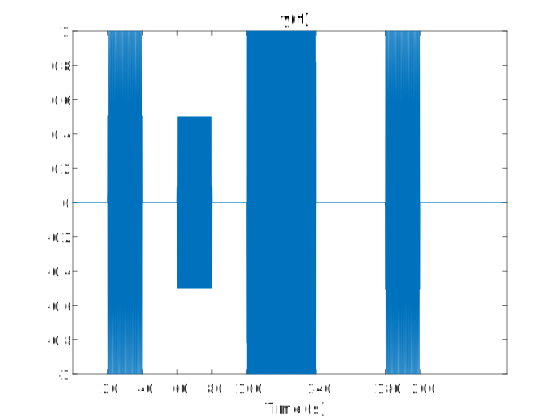
\includegraphics[width=0.4\textwidth]{Img/pulseSignal.eps}
	\caption[Pulse Signal]{Example of pulse signal}
	\label{examplePulseSignal}
\end{figure}

Once the signal has been defined and constructed, it is played and recorded by the class \class{ReproductorRecorder}. The recorded signal is of course different from the transmitted one. It has been modified by the response of loudspeakers and microphones, the noise, the directivity, position of objects, etc. However, we must detect the pulses in order to calculate how the amplitude and phase has been modified. So, how is the detection performed?

\subsection{Detection of pulses}
We take advantage of the fact that we know what the transmitted signal is. So what we are interested in is not detecting the frequency, which we already know, but the complex coefficients of each pulse.

The first step is then to calculate the IQ signal, this is, the low frequency signal that modulates the carrier, whose frequency we know. The relation of the IQ signal and the original one is:
\begin{equation}
x(t) = \Re\{ e^{j 2 \pi f t} x_{IQ}(t) \} = |x_{IQ}(t)| \cos(2 \pi f t + \phi(t))
\label{IQcondition}
\end{equation}
It can be done by applying a band-pass filter around the desired frequency and down-converting the resulting signal (\reffig{detectionScheme}).
\begin{figure}[h]
	\centering
	\includegraphics[width=0.9\textwidth]{Img/detectionScheme.pdf}
	\caption[Detection Scheme]{Scheme of the detection}
	\label{detectionScheme}
\end{figure}

Now that we have the modulating signal $x_{IQ}(t)$, we need to detect where the pulses are. Their amplitude and phase can change, and they can be distorted by noise and non-linear effects, but the duration and delay between them is going to be approximately the same. Hence, we can generate a mask that is set to one when there is a pulse in the original signal and to zero otherwise, cross-correlate it by $x_{IQ}(t)$, and find the lag that returns the maximum value of correlation. To find the complex coefficients of pulses (amplitude and phase), we just perform the mean of each pulse.

\subsection{Calibration}
However, there is a problem that must be solved. Calibration...

%%\section{Overview of the system}
The program WFSTool was develop as a GUI that helps to use WFS in the lab. It was developed in its original version by YU Bofei as part of her undergraduate project, and has been modified by me.

The last version of the program is developed using the object-oriented programming capability of Matlab. The architecture is modular. There is the parent object, which contains all the other objects as properties. In the next sections a detailed explanation of each of the objects will be given.

\section{Reproductor}
The class \textit{reproductor} is the core of the whole system. It is a system object that interacts with the audio card of the computer and controls the processing and reproduction of the audio files.

It has no public properties, so every property must be set using the public functions. The properties that allow the user to configure the object are the next nontunnable properties:

\begin{enumerate}
	\item 'audioFileName'. Use the function \textit{executeOrder(order)}. \textit{order} is a structure where the field \textit{action} 'assignTrack' and the field \textit{fileName} is the name of the audio track.
	\item 'frameSize'. Use the function \textit{setFrameSize(frameSize)}.
	\item 'driver'. Use the function \textit{setDriver(driver)}.
	\item 'device'. Use the function \textit{setDevice(device)}.
	\item 'getDelayFun'. Use the function \textit{set\_getDelayFun(getDelayFun)}.
	\item 'getAttenFun'. Use the function \textit{set\_getAttenFun(getAttenFun)}.
\end{enumerate}

There are two properties that the user cannot change, but are informative about the current state of the object and can be used during the interaction with other objects.

\begin{enumerate}
	\item 'playingState'. It can have 3 values: \textit{playing}, \textit{paused} and \textit{stopped}.
	\item 'numChannels'. Number of output channels, this is, the number of channels of the output buffer. The delay and attenuation returned by the getDelayFun and getAttenFun must match this number. It is not necessarily the real number of output channels of the output audio device, but the number of channels that the object is feeding to the driver, this is, the number of channels the object believes there are.
\end{enumerate}

Finally, there are internal properties to which the user has no access.

The rest of the interaction that the user or other objects can have with an object of the class \textit{reproductor} are the construction with the function \textit{reproductor} and the reproduction control by means of the function \textit{executeOrder(order)}.

The constructor doesn't admit any input arguments, so there is not much to say about it.

The reproduction control is more complex though. The function \textit{executeOrder(order)} accepts one parameter (\textit{order}) that must be a structure with at least one field called \textit{action} and, optionally, another one called \textit{fileName}. The field \textit{action} defines the action that it is required to execute, but the taken steps vary depending on the \textit{playingState}:


\subsection*{\textit{playingState} = 'playing'}
\begin{description}
	\item[play] The required action is to start reproducing an audio track. If the field \textit{fileName} exists, it will become the new \textit{audioFileName}. If not, the song that will start to reproduce is the current \textit{audioFileName}.
	\item[stop] Stop the reproduction of any song and release the object.
	\item[pause] Pause the reproduction of the audio track, but don't release the object, so the nontunable properties are still nontunable.
	\item[resume] Do nothing.
	\item[assignTrack] The same as \textit{play}.
\end{description}

\subsection*{\textit{playingState} = 'paused'}
\begin{description}
	\item[play] The same as in the 'playing' state.
	\item[stop] Stop the reproduction of any song and release the object.
	\item[pause] Do nothing since the object is already paused.
	\item[resume] Resume the reproduction of the audio track.
	\item[assignTrack] Stops the reproduction and then updates the property \textit{audioFileName}.
\end{description}

\subsection*{\textit{playingState} = 'stopped'}
\begin{description}
	\item[play] The same as in the 'playing' state.
	\item[stop] Do nothing as the object is already stopped.
	\item[pause] Do nothing, it makes no sense since nothing is being reproduced.
	\item[resume] The same as \textit{play} if there was no \textit{fileName} specified, i.e., just start reproducing the current \textit{audioFileName}.
	\item[assignTrack] It updates the property \textit{audioFileName}.
\end{description}

Additionally, the content of the field \textit{action} can be an empty string, in which case no action is performed. Any other content of the field will throw an error.

\section{Reproduction panel}
The reproduction panel consists of a panel like the one in Fig.\ref{}. Each time the user interacts with it, the object executes a callback externally specified with an order structure as the first argument. There are also public functions for updating the state of the panel.

The panel stores a list of audio tracks, and the selected audio track and the active audio track.

The order structure has two fields:
\begin{enumerate}
	\item 'action'. It is the action. It can be of the type:
	\begin{enumerate}
		\item 'play'
		\item 'stop'
		\item 'pause'
		\item 'next'
		\item 'previous'
		\item 'doubleClick'
	\end{enumerate}
	\item 'fileName'. In case it is needed, it is the name of the audio file associated with the action. It can be the file that is currently active, or the one that is selected.
\end{enumerate}

\chapter{Analysis of potential sources of error}
%\section{Experiment 1: theoretical simulation}
As we've seen before, the loudspeaker array in the laboratory can be modelled as an octagon of monopoles (\autoref{WFSdistribution}). If a monopole source is placed outside the area, the loudspeaker array should be able to replicate the field with opposite sign and hence, cancel it inside the octagon. As explained in \autoref{optimization}, the election of points matters when applying the global scalation of loudspeaker coefficients (\autoref{OptScalation}). Therefore, a more or less even distribution of points should be chosen.

As an example, \autoref{figTheoCanc} shows the result for a noise source at position $[-1, 2.5, 0]$, and the optimization applied for the points represented by microphone icons. The frequency from now on is $440\si{Hz}$ unless it is explicitly mentioned otherwise.

\begin{figure}[H]
	\centering
	\reflectbox{\rotatebox[origin=c]{180}{
			\includegraphics[height=0.3\textheight]{./Img/Experiment1_Example_definitive.pdf}
	}}	
	\caption[WFS cancellation]{WFS cancellation. $\pos[vecNS]{} = [-1, 2.5, 0]$.}
	\label{figTheoCanc}
\end{figure}

To get a sense of what levels of cancellations we can achieve, we test it for different positions of the noise source (\autoref{figNoiseSourcePosTheo}), and the results are shown in \autoref{figCancelDiffNSpostheo}. We've used \autoref{globalCancEq} to calculate the cancellation. As we can see, the closer the noise source is to the centre of the silent area, the better the cancellation. The further it is located, the worse levels of cancellation achieved, but it seems it converges when $R\rightarrow\infty$ to cancellations over $11$ dB. As this is the ideal case, it's reasonable to don't expect better performance in real cases.

\begin{figure}[h]
	\centering
%	\raisebox{0.1\height}{
	\begin{minipage}[b]{0.49\textwidth}
			\centering
			\def\svgwidth{\columnwidth}
			\graphicspath{{Img/}}
			\input{Img/Experiment1_differentNSpositions.pdf_tex}
			\caption[Positions of noise source]{Positions of noise source}
			\label{figNoiseSourcePosTheo}
	\end{minipage}
	\begin{minipage}[b]{0.49\textwidth}
			\centering
		\includegraphics[width=\textwidth]{Img/Experiment1_globalCancDifNSpos_definitive.pdf}
		\caption[Global cancellation. Theoretical model.]{Global cancellation for different positions of the noise source.}
		\label{figCancelDiffNSpostheo}
	\end{minipage}
\end{figure}

%% Comentado el 9/4/2018 porque creo que ya sabiendo de dónde sale la 2.5D Rayleigh I integral, no tiene sentido seguir evaluando esto.
%Respect to the global correction factor $\Psi$ (\autoref{OptScalation}), in \autoref{figGobalScalationScatter} we can see that, although it changes with distance $R$ and angle $\alpha$, the variation is very small. The mean absolute value is around $0.21$ and the mean phase is approximately $-137^\circ$. 
%
%\begin{figure}[H]
%	\centering
%	\includegraphics[height=0.3\textheight]{./Img/Experiment1_globalCancScaleFactor.eps}
%	\caption[Global correction factor]{Global correction factor}
%	\label{figGobalScalationScatter}
%\end{figure}
%
%One question that may arise is how much the election of microphones location can change the value of the optimal global scale factor $\Psi$, and so, the cancellation. In order to evaluate that change, we define a new magnitude. Let $\Psi_{\mathit{opt}, i}$ be the optimal global cancellation factor for a given microphone distribution $\pos[matMicro]{,i}$ (\autoref{corrFacti}). Let's define $\cmicro[(i,j)]$ (\autoref{cmicroDifferentPsi}) as the signals received by a set of microphones located at $\pos[matMicro]{,i}$ and correction factor $\Psi_{\mathit{opt}, j}$ (calculated with a different set of microphone locations $\pos[matMicro]{,j}$). Now, we can define $C_{\mathit{global}(i,j)}$ as the global cancellation achieved with $\cmicro[(i,j)]$ (\autoref{globCancOther}).
%
%\begin{gather}
%\Psi_{\mathit{opt}, i} = \argmin_{\Psi} \norm{\Awfs(\pos[matMicro]{,i})\cwfs \Psi + \vec{a}_{\mathit{NS}}(\pos[matMicro]{,i}) \cnsScalar} \label{corrFacti} \\
%\cmicro[(i,j)] = \Awfs(\pos[matMicro]{,i})\cwfs \Psi_{\mathit{opt}, j} + \vec{a}_{\mathit{NS}}(\pos[matMicro]{,i}) \cnsScalar \label{cmicroDifferentPsi} \\
%C_{\mathit{global}(i,j)} = \frac{\norm{\cmicro[(i,j)]}^2}{\norm{\vec{a}_{\mathit{NS}}(\pos[matMicro]{,i}) \cnsScalar}^2} \label{globCancOther}
%\end{gather}
%
%Different sets of microphone locations have been chosen \autoref{figGrids}. All of them are rectangular grids with dimensions ($2.1$x$3.8$)$\si{m}$, but the number of rows and columns change. The global correction factor has been calculated for all of them for different positions of the noise source and radius $R = 50\si{m}$, and the global cancellation $C_{\mathit{global}(i,j)}$ for the last grid (the most complete one) is shown in \autoref{figDiffMicroGridsCanc}. We can notice that just one microphone situated at the centre of the octagon (grid a) is not enough to calculate a correction factor $\Psi$ that would produce good cancellations. However, a grid of just 9 microphones (grid b) already achieves cancellation levels just $2\si{dB}$ worse than the better case (grid e), which can mean that not many microphones inside the area would be needed to scale correctly the transmitted signals.
%
%\begin{figure}[H]
%	\centering
%	\begin{subfigure}[b]{0.3\textwidth}
%		\centering
%		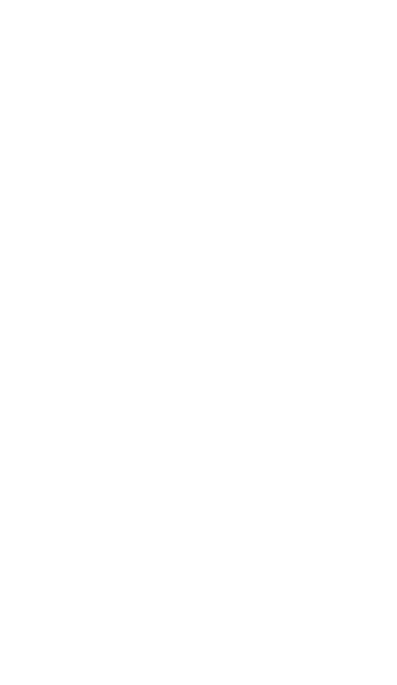
\includegraphics[width=0.75\textwidth]{./Img/Experiment1_imageGrid1.pdf}
%		\caption{1 microphone}
%	\end{subfigure}
%	\begin{subfigure}[b]{0.3\textwidth}
%		\centering
%		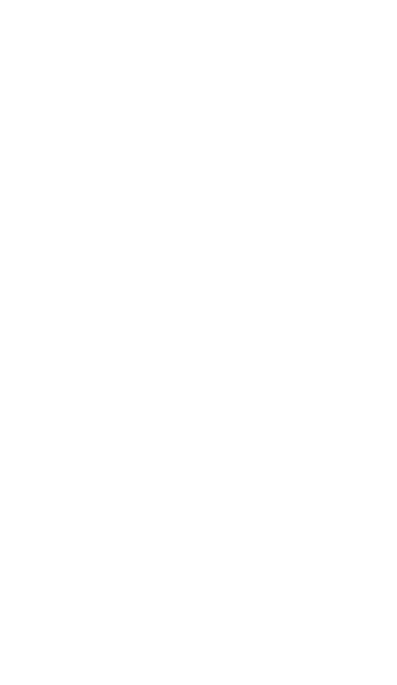
\includegraphics[width=0.75\textwidth]{./Img/Experiment1_imageGrid2.pdf}
%		\caption{(3x3)}
%	\end{subfigure}
%	\begin{subfigure}[b]{0.3\textwidth}
%		\centering
%		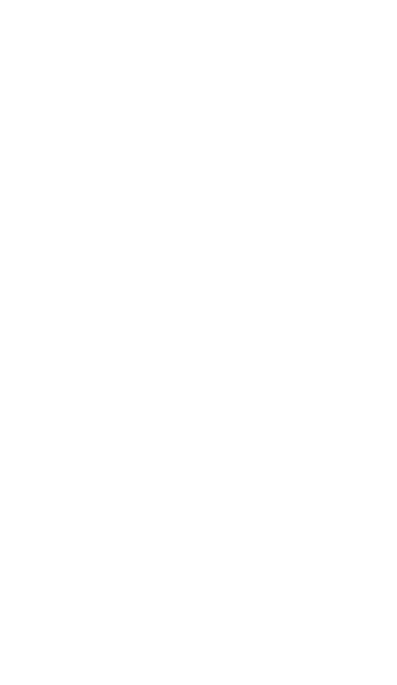
\includegraphics[width=0.75\textwidth]{./Img/Experiment1_imageGrid3.pdf}
%		\caption{(5x5)}
%	\end{subfigure}
%	\begin{subfigure}[b]{0.3\textwidth}
%		\centering
%		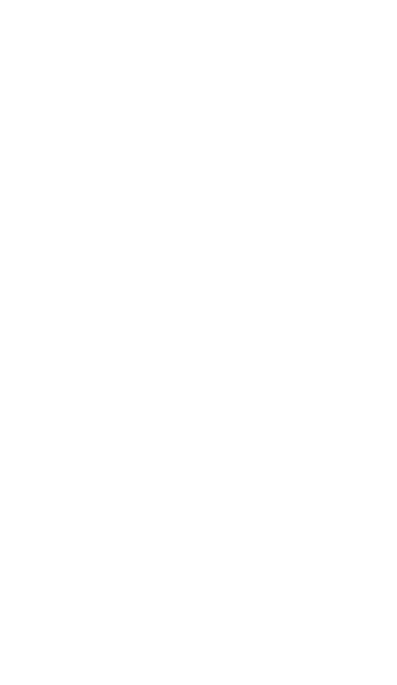
\includegraphics[width=0.75\textwidth]{./Img/Experiment1_imageGrid4.pdf}
%		\caption{(10x10)}
%	\end{subfigure}
%	\begin{subfigure}[b]{0.3\textwidth}
%		\centering
%		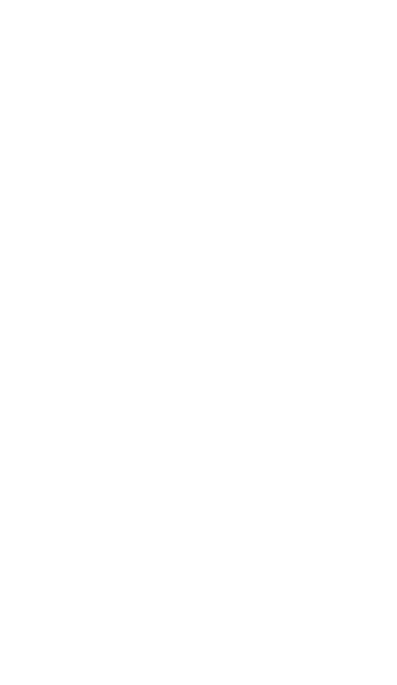
\includegraphics[width=0.75\textwidth]{./Img/Experiment1_imageGrid5.pdf}
%		\caption{20x20}
%	\end{subfigure}
%	\caption{Grids for microphone positions}
%	\label{figGrids}
%\end{figure}
%
%\begin{figure}[H]
%	\centering
%	\includegraphics[height=0.4\textwidth]{./Img/Experiment1_diffMicroGrid.eps}
%	\caption[Global cancellation for different number of microphones]{Global cancellation for different number of microphones}
%	\label{figDiffMicroGridsCanc}
%\end{figure}

Another question worth studying is what happens when the noise source is not in the same plane as the WFS loudspeaker array, this is, when the $z$ coordinate is not 0. In \autoref{figGlobCancDifNSz} there is represented the global cancellation with respect to the angle $\theta$ between the horizontal plane and the vector that goes from the centre of the array to the noise source (\autoref{figDifNSz}). We can see that the lost in cancellation levels starts getting very big for angles $\theta > 15^\circ$.

\begin{figure}[H]
	\centering
	\begin{subfigure}[b]{0.49\textwidth}
	\centering
	\def\svgwidth{\columnwidth}
	\graphicspath{{Img/}}
	\input{Img/Experiment4_diffNSzpos_definitive.pdf_tex}
	\caption{Scheme}
	\label{figDifNSz}
	\end{subfigure}
	\begin{subfigure}[b]{0.49\textwidth}
	\centering
	\includegraphics[width=\columnwidth]{Img/Experiment4_globalCancDifNSz.eps}
	\caption{Global cancellation for different $z$ positions of the noise source}
	\label{figGlobCancDifNSz}
\end{subfigure}
	\caption{Noise source outside WFS array plane}
\end{figure}

Finally, it's worth noting that, although previously we have described a type of optimization (\autoref{optNoRestrictions}) that would consist in just solving a linear system without the use of WFS theory, it's actually not a useful method. The reason why it's not is because the solution it finds requires some of the secondary loudspeakers to transmit signals with an amplitude hundreds of times bigger than the amplitude of the noise signal, as it was noted in \cite{Lapini2016}. Moreover, the density of microphone locations needed to achieve good cancellation levels over the whole area is significantly bigger than in the global correction case \autoref{figNoConst}. In conclusion, WFS theory is necessary.

\begin{figure}[H]
	\centering
	\begin{subfigure}[b]{0.49\textwidth}
		\centering
		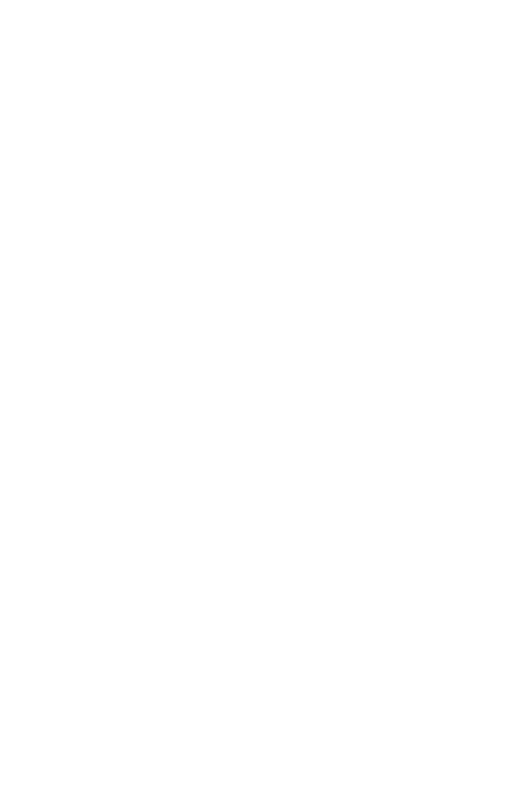
\includegraphics[width=0.75\textwidth]{./Img/Experiment1_noConstOpt_grid3.pdf}
		\caption{}
	\end{subfigure}
	\begin{subfigure}[b]{0.49\textwidth}
		\centering
		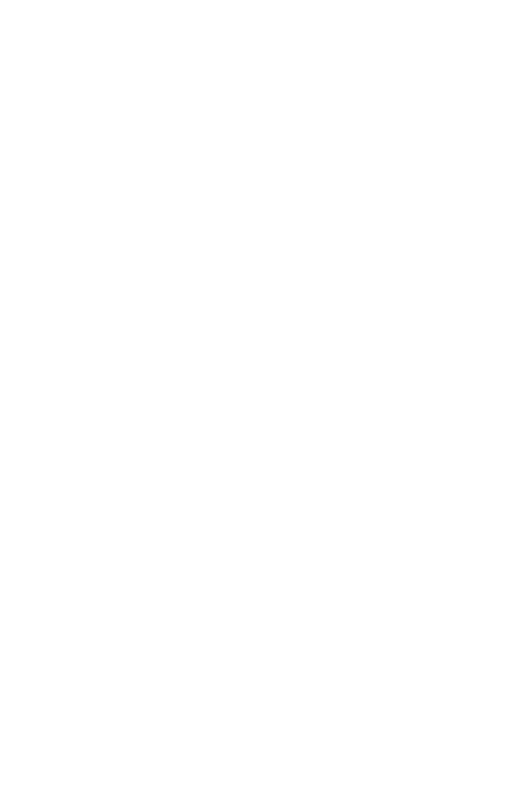
\includegraphics[width=0.75\textwidth]{./Img/Experiment1_noConstOpt_grid5.pdf}
		\caption{}
	\end{subfigure}
	\caption{Optimization without WFS}
	\label{figNoConst}
\end{figure}

\section{Experiment 2: GTAC acoustic paths}
These experiment is also a theoretical one, although it uses results from previous measures. The acoustic responses in the GTAC anechoic chamber for different points was measured with high precision previously, and the results are published in the website \cite{GTACroom}. The measures were done in 360 points distributed in a rectangular grid of size $24$x$15$ and separation of $20 \si{cm}$ between adjacent nodes (\autoref{GTAC360micro}).

GTAC responses are measured for loudspeakers in the WFS array, but of course, not for loudspeakers outside the array in arbitrary positions. Hence, we can only guess the acoustic paths by applying the theoretical model (\autoref{acPathTheoric}), in which case we assume that the noise source is isotropic.

Results are shown in \autoref{figGTACglobalCancAlltogether}. Different positions have been used. As we can see, the cancellation levels are quite far from the theoretical case.

\begin{figure}[H]
	\begin{minipage}[b]{0.49\textwidth}
		\centering
		\reflectbox{\rotatebox[origin=c]{180}{
				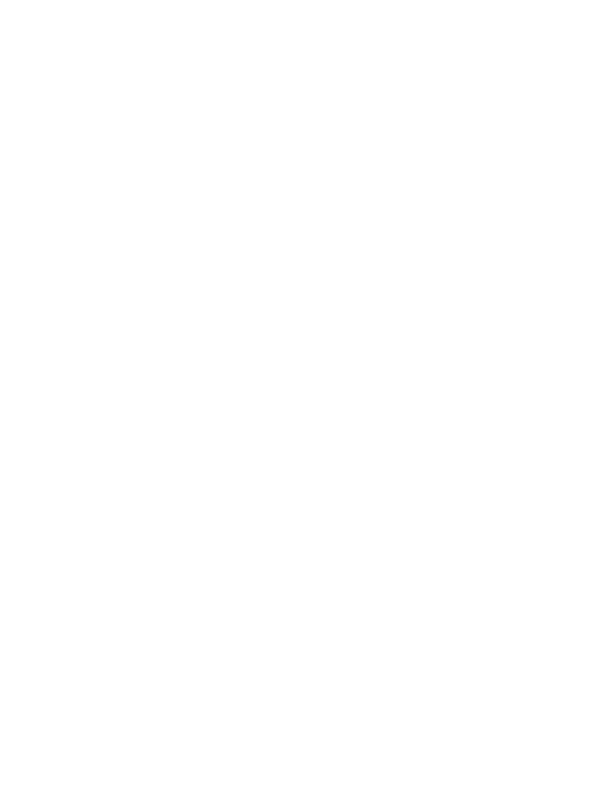
\includegraphics[height=0.8\textwidth]{./Img/WFSGTAC360microphones.pdf}
		}}	
		\caption[Schematic of measures in GTAC anechoic chamber]{Schematic of measures in GTAC anechoic chamber}
		\label{GTAC360micro}
	\end{minipage}
	\begin{minipage}[b]{0.49\textwidth}
	\centering
	\includegraphics[height=0.8\textwidth]{./Img/Experiment2_globalCancDifNSpos_definitive.pdf}	
	\caption[Global cancellation for GTAC impulse responses]{Global cancellation for GTAC impulse responses}
	\label{figGTACglobalCancAlltogether}
\end{minipage}
\end{figure}

The reason for this can be found when we take a look at the impulse response of each individual loudspeaker. For example, let's focus on the loudspeaker number $20$. If we were in the ideal case and feeded the loudspeaker with a signal of amplitude $1$, the amplitude and phase of the signals at each measure point would be the one shown in \autoref{figGTAClouds20idealCaseAbs} and \autoref{figGTAClouds20idealCasePhase} . Instead, what we find in the measured acoustic response is slightly different (\autoref{figGTAClouds20realCaseAbs} and \autoref{figGTAClouds20realCasePhase}).

\begin{figure}[H]
	\centering
	\begin{subfigure}[b]{0.24\textwidth}
		\centering
		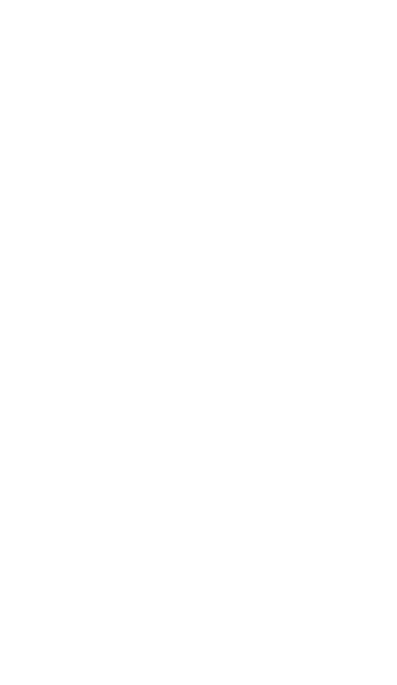
\includegraphics[width=0.75\textwidth]{./Img/Experiment2_loud20_IdealAbsMap.pdf}
		\caption{Ideal case. Amplitude.}
		\label{figGTAClouds20idealCaseAbs}
	\end{subfigure}
		\begin{subfigure}[b]{0.24\textwidth}
		\centering
		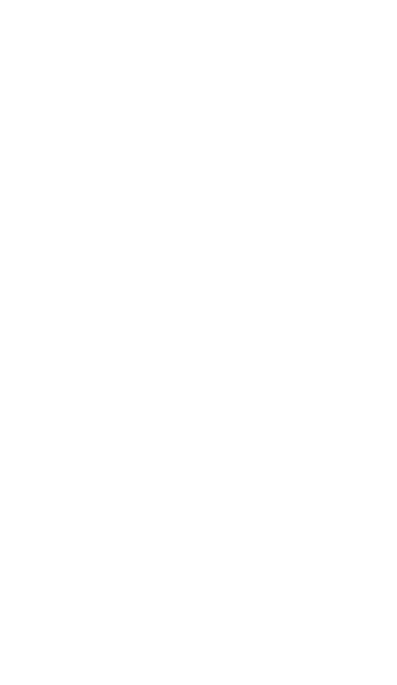
\includegraphics[width=0.75\textwidth]{./Img/Experiment2_loud20_RealAbsMap.pdf}
		\caption{Real case. Amplitude.}
		\label{figGTAClouds20realCaseAbs}		
	\end{subfigure}
	\begin{subfigure}[b]{0.24\textwidth}
		\centering
		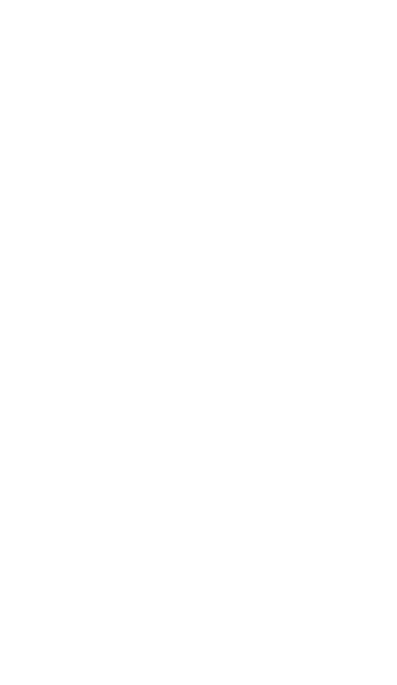
\includegraphics[width=0.75\textwidth]{./Img/Experiment2_loud20_IdealPhaseMap.pdf}
		\caption{Ideal case. Phase.}
		\label{figGTAClouds20idealCasePhase}
	\end{subfigure}
	\begin{subfigure}[b]{0.24\textwidth}
		\centering
		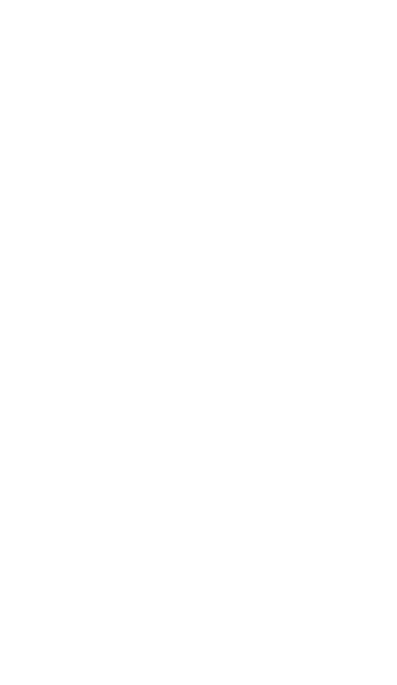
\includegraphics[width=0.75\textwidth]{./Img/Experiment2_loud20_RealPhaseMap.pdf}
		\caption{Real case. Phase.}
		\label{figGTAClouds20realCasePhase}
	\end{subfigure}
	\caption{Loudspeaker number 20 acoustic paths.}
	\label{figGTAClouds20}
\end{figure}

In order to get a sense of how different the ideal and real cases are, in \autoref{figGTAClouds20Comparison} we have represented in a graph the amplitude and phase shift (measured phase minus the theoretical one) of the field as a function of the distance to the loudspeaker. For the theoretical case, the amplitude is inversely proportional to the distance, and the phase is linear. However, for the measured acoustic paths, there is a cloud of scattered points in both cases, being the scattering bigger as the distance increases. A similar behaviour is found for all the other loudspeakers.

\begin{figure}[H]
	\begin{subfigure}[b]{0.49\textwidth}
		\centering
		\includegraphics[height=0.8\textwidth]{./Img/Experiment2_loud20_AmpByDist.eps}
		\caption{Amplitude}
	\end{subfigure}
	\begin{subfigure}[b]{0.49\textwidth}
		\centering
		\includegraphics[height=0.8\textwidth]{./Img/Experiment2_loud20_PhaseByDist.eps}
		\caption{Phase}
	\end{subfigure}
	\caption{Amplitude and phase of field as a function of distance for loudspeaker number 20.}
	\label{figGTAClouds20Comparison}
\end{figure}

An upper bound to the global cancellation achievable can be calculated using the optimization without any constraints expressed in \autoref{optNoRestrictions}. Results are shown in \autoref{figGTACmaxGlobCancNoConst}. As we can see, the best cancellation levels we can achieve are not better than $7\si{dB}$ in most cases.

\begin{figure}[H]
	\centering
	\includegraphics[height=0.5\textwidth]{./Img/Experiment2_globalCancDifNSposNoConst_definitive.pdf}
	\caption{Global cancellation for GTAC impulse responses. Optimization without constraints.}
	\label{figGTACmaxGlobCancNoConst}
\end{figure}

\section{Experiment 3: lab recording}
Completar

\section{Introduction}
In the GTAC anechoic chamber there is a 96-loudspeaker array distributed as an irregular octagon in the horizontal plane (\autoref{WFSdistribution}), $1.65 \si{m}$ above the floor, with a separation between loudspeakers of $\secondarySourceSeparation = 0.18 \si{m}$. 

Many variables have an impact on the acoustic field generated by the loudspeakers: frequency dependent directivity of each individual loudspeaker, non-linearities, reverberation of the chamber, diffraction, reflections on the floor (which is not recovered with absorbing material as the walls), etc. However, if we assume a simple model where the anechoic chamber is perfectly configured to emulate free-space conditions, and every loudspeaker is identical to the rest and behaves as an ideal monopole, then the similarities with the scenario presented by WFS theory become clear.

Under ideal conditions, the octagon can be interpreted as the closed curve of secondary sources $\sectionTheo$ discretized with a step of $\secondarySourceSeparation = 0.18 \si{m}$. As we only count with monopole sources (loudspeakers with dipole characteristics are more difficult and expensive to manufacture), we should use the Rayleigh 2.5D I integral (\autoref{RayleighI2.5}), but $\sectionTheo$ should be an infinite line and not an octagon. Of course, in practice an infinite array is not realizable, so at some point we must truncate the array anyway. On the other hand, when dealing with a bent array, the amplitude factor $g = \sqrt{\frac{d}{d + \abs{\PosTheo[primarySource][z]}}}$ that was calculated when $\sectionTheo$ was a straight line might not be the best option any more.

The actual loudspeaker feeding signals that were used, were calculated applying formulas that were provided by the professors and are particularized for the specific geometry of the GTAC array:
\begin{equation}
\begin{aligned}
g &= 
\begin{cases}
\sqrt{\frac{\distLinePoint}{\distLinePrimSource + \distLinePoint}} & \normPrimaryPropAngle \leq 90^\circ \\
0 & \normPrimaryPropAngle > 90^\circ
\end{cases}
\\
\distLinePoint &= \frac{1.44}{2} + 1.44 \cos\left( \frac{\pi}{4} \right)
\end{aligned}
\label{amplitFactorGTAC}
\end{equation}

\section{Simulation 1}
Traditionally, WFS has been used, not to cancel noise, but as a spatial audio reproduction system that competes with existing stereophonic systems as Dolby Surround. The main focus has been, then, not in replicating accurately a field, but in generating the subjective impression of natural hearing, this is, of sound heard from various directions. So, the evaluation of performance has been usually guided by the ability of subjects to localize virtual sound sources and other subjective measures.

Since human hearing has limitations, there are objective sound characteristics that it cannot perceive. We can take advantage of this, and use compression, downsampling and other techniques (common in mp3 and other compression formats) that lower the requirements of the system without worsening the subjective perception. One thing that humans cannot distinguish is


\chapter{Experimental measures}
WFS theory is based on a propagation model where the acoustic field is generated by punctual primary sources and the cancellation field is generated by punctual monopole secondary sources, everything in an homogeneous media and free-space condition, and the location of every source is perfectly known.

A real situation, as the one we find in a listening room with real loudspeakers, is very different. A great variety of phenomena not contemplated by the WFS simple model occur: reflections, diffractions produced by obstacles, loudspeakers are not punctual sources so the near-field does not follow the far-field approximation, the directivity is not the one of an ideal monopole and depends on the frequency, the frequency response of loudspeakers is not flat, which would not be that big of a problem if it was the same for every loudspeaker, but it might actually be very different from one to the other, their exact locations are not accurately known, non-linearities, etc.

All these differences influence the way the acoustic waves propagate and, in general, they worsen the performance in a real situation. Experimental measures help us understand how this not contemplated differences limit the possibilities of using WFS in the real world.
\begin{shownto}{private}
\section{Acoustic path model}
In order to find a connection between the real and ideal situation, let's use a model of what is happening.
\end{shownto}
In a real situation, all we can certainly know is that, if we transmit a signal through a loudspeaker and we measure at some point with a microphone, we receive a modified version of the signal. That modification depends on all the conditions previously mentioned (multiple reflections, etc.), and together they form what is often called acoustic path. An acoustic path between a loudspeaker and a point of measure acts as a filter characterized by an impulse response (time domain) or frequency response (frequency domain).

The relation between the transmitted signals and the received ones in the frequency domain is:
\begin{shownto}{private}
\begin{equation}
\Field[noValue][frequency][vector](f) = \AcPath[mat](f) \vec{\signal[nothing][frequency]}(f) ,
\end{equation}
where $\Field[noValue][frequency][vector] = [\Field[noValue][frequency][scalar]_1, \Field[noValue][frequency][scalar]_2, ..., \Field[noValue][frequency][scalar]_\numMeasPoints]^T$ ($\numMeasPoints$ is the number of points of measure) is the acoustic pressure vector, $\vec{\signal[nothing][frequency]} = [\signal[nothing][frequency]_1, \signal[nothing][frequency]_2, ..., \signal[nothing][frequency]_\numSources]^T$ ($\numSources$ is the number of loudspeakers) is the transmitted signals vector, and $\AcPath[mat]_{(\numMeasPoints \times \numSources)}$ is a matrix whose $(m,n)$-th element is the frequency response of the acoustic path between the $n$-th loudspeaker and the $m$-th point of measure.

When we differentiate the noise sources and the WFS array sources:
\begin{multline}
\Field[noValue][frequency][vector](f)
= \left. \begin{cases}
\vec{\signal[nothing][frequency]} = 
\begin{bmatrix}
\vec{\signal[wfs][frequency]} \\
\vec{\signal[ns][frequency]}
\end{bmatrix} \\
\AcPath[mat] =
\begin{bmatrix}
\AcPath[mat][WFS], & \AcPath[mat][NS]
\end{bmatrix}
\end{cases} \right\} \\
 = \AcPath[mat][NS](f) \vec{\signal[ns][frequency]}(f) + \AcPath[mat][WFS](f) \vec{\signal[wfs][frequency]}(f)
 = \Field[ns][frequency][vector](f) + \Field[wfs][frequency][vector](f),
\end{multline}
where $\Field[ns][frequency][vector] = [\Field[ns][frequency][scalar][1], \Field[ns][frequency][scalar][2], ..., \Field[ns][frequency][scalar][\numMeasPoints]]^T$, $\Field[wfs][frequency][vector] = [\Field[wfs][frequency][scalar][1], \Field[wfs][frequency][scalar][2], ..., \Field[wfs][frequency][scalar][\numMeasPoints]]^T$, $\vec{\signal[ns][frequency]} = [\signal[ns][frequency]_1, \signal[ns][frequency]_2, ..., \signal[ns][frequency]_{\numNS}]^T$ ($\numNS$ is the number of noise sources), $\vec{\signal[wfs][frequency]} = [\signal[wfs][frequency]_1, \signal[wfs][frequency]_2, ..., \signal[wfs][frequency]_{\numWFS}]^T$ ($\numWFS$ is the number of secondary sources) and $\AcPath[mat][NS]$ and $\AcPath[mat][WFS]$ are the acoustic path matrices of the noise sources and WFS secondary source array respectively. If the cancellation is successful, $\Field[ns][frequency][vector](f) \approx -\Field[wfs][frequency][vector](f)$ and so, $\Field[noValue][frequency][vector]$ becomes really small.
\end{shownto}

\begin{shownto}{public}
\begin{multline}
	\Field[noValue][frequency][vector](f)
	= \AcPath[mat](f) \vec{\signal[nothing][frequency]}(f)
	= \left. \begin{cases}
		\vec{\signal[nothing][frequency]} = 
		\begin{bmatrix}
			\vec{\signal[wfs][frequency]} \\
			\vec{\signal[ns][frequency]}
		\end{bmatrix} \\
		\AcPath[mat] =
		\begin{bmatrix}
			\AcPath[mat][WFS], & \AcPath[mat][NS]
		\end{bmatrix}
	\end{cases} \right\} \\
	= \AcPath[mat][NS](f) \vec{\signal[ns][frequency]}(f) + \AcPath[mat][WFS](f) \vec{\signal[wfs][frequency]}(f)
	= \Field[ns][frequency][vector](f) + \Field[wfs][frequency][vector](f),
	\label{acPathModel}
\end{multline}
where $\Field[ns][frequency][vector] = [\Field[ns][frequency][scalar][1], \Field[ns][frequency][scalar][2], ..., \Field[ns][frequency][scalar][\numMeasPoints]]^T$ and $\Field[wfs][frequency][vector] = [\Field[wfs][frequency][scalar][1], \Field[wfs][frequency][scalar][2], ..., \Field[wfs][frequency][scalar][\numMeasPoints]]^T$ are the acoustic pressure vectors ($\numMeasPoints$ is the number of points of measure), $\vec{\signal[ns][frequency]} = [\signal[ns][frequency]_1, \signal[ns][frequency]_2, ..., \signal[ns][frequency]_{\numNS}]^T$ ($\numNS$ is the number of noise sources) and $\vec{\signal[wfs][frequency]} = [\signal[wfs][frequency]_1, \signal[wfs][frequency]_2, ..., \signal[wfs][frequency]_{\numWFS}]^T$ ($\numWFS$ is the number of secondary sources) are the transmitted signal vectors, and ${\AcPath[mat][NS]}_{(\numMeasPoints \times \numNS)}$ and ${\AcPath[mat][WFS]}_{(\numMeasPoints \times \numWFS)}$ are matrices whose $(m,n)$-th element is the frequency response of the acoustic path between the $n$-th loudspeaker and the $m$-th point of measure. If the cancellation is successful, $\Field[ns][frequency][vector](f) \approx -\Field[wfs][frequency][vector](f)$ and so, $\Field[noValue][frequency][vector]$ becomes really small. Cancellation will be successful as long as the acoustic paths are the same or very similar to the ideal ones. In the ideal case, the $(m,n)$-th element of $\AcPath$ would apply a simple delay and an amplitude attenuation:
\begin{equation}
a_{m,n}(f) = \frac{e^{-j k d_{m,n}}}{d_{m,n}},
\end{equation}
where $d_{m,n}$ is the distance between the $n$-th loudspeaker and the $m$-th point of measure.
\end{shownto}

\begin{shownto}{private}
The signal reproduced by the secondary loudspeakers $\vec{\signal[wfs][frequency]}$ depends on the noise source signals $\vec{\signal[ns][frequency]}$. Specifically, each secondary source filters the noise source signals, as it was expressed in \autoref{rayleigh2_5Dsignal} and rewritten here:
\begin{multline}
\signal[wfs][frequency](f) = \signal[nsVirt][frequency](f) \frac{g \cos\normPrimaryPropAngleSection}{\sqrt{\distLinePrimSource}}
e^{-j k \distLinePrimSource} \sqrt{\frac{jk}{2\pi}} = \\
\left\{
\signal[nsVirt][frequency](f) = -\signal[ns][frequency] \rightarrow
H(f) = -\frac{g \cos\normPrimaryPropAngleSection}{\sqrt{\distLinePrimSource}}
e^{-j k \distLinePrimSource} \sqrt{\frac{jk}{2\pi}}
\right\} = \signal[ns][frequency](f) H(f).
\end{multline}
Expressed as a matrix multiplication:
\begin{equation}
\vec{\signal[wfs][frequency]} = \myMatrix{H} \vec{\signal[ns][frequency]},
\end{equation}
where $\myMatrix{H}_{\numWFS \times \numNS}(f)$ is a matrix where the $(m,n)$-th element is the filter frequency response that the $m$-th array loudspeaker applies to the $n$-th noise source.

In the model assumed by WFS theory (free-space conditions, ideal monopole point sources), the acoustic path response between a source and a point of measure separated by a distance $d$ is:
\begin{equation}
a(f) = \frac{e^{-j k d}}{d}.
\end{equation}
This allows us to construct $\AcPath[mat]'(f)$, the acoustic path response matrix for ideal conditions. The $(m,n)$-th element would be 
\begin{equation}
a_{m,n}'(f) = \frac{e^{-j k d_{m,n}}}{d_{m,n}},
\end{equation}
where $d_{m,n}$ is the distance between the $n$-th loudspeaker and the $m$-th point of measure.

Under these conditions, good cancellation levels can be achieved. The actual $\AcPath[mat]$ includes all sorts of variations, as we saw, so one could expect the experimental result to be much worse than what theory predicts.
\end{shownto}

\begin{shownto}{private}
\section{Volume correction}
However, a way of making this model more realistic is by adding a variable that accounts for the possible sound volume difference between the noise source and the secondary loudspeaker array. This is useful because in the listening room we generate the noise signal with a loudspeaker. Unlike the secondary array loudspeakers, which were all adjusted to have similar behaviour, the noise loudspeaker volume can be independently adjusted manually. If we change it for another loudspeaker, the volume might be actually very different. This introduces an unknown variable that definitely affects cancellation, but it's really easy to model and compensate.

Basically, regarding the volume of the source as a separate variable when dealing with real loudspeakers, force us to differentiate between the digital signal in arbitrary units $\signal[nothing][frequency]$, and the real signal in acoustic pressure units (for example, Pascals) $\soundVolume \signal[nothing][frequency]$, where $\soundVolume$ is the sound volume of the loudspeaker that transforms arbitrary units in pressure units. This term goes then included in the acoustic path matrix $\AcPath[mat]$, where the $n$-th column is multiplied by the volume associated to the $n$-th loudspeaker. Since we consider that all loudspeakers of the secondary array are well calibrated and, for simplification purposes, also considering all noise loudspeakers have the same volume:
\begin{equation}
\Field[noValue][frequency][vector]
= (\soundVolume[ns]\AcPath[mat][NS]' + \soundVolume[wfs]\AcPath[mat][WFS]'\myMatrix{H}) \vec{\signal[ns][frequency]},
\end{equation}
where $\AcPath[mat][NS]'$ and $\AcPath[mat][WFS]'$ are the ideal acoustic path matrices when the volume term is not included. This means that $\AcPath[mat][NS] = \soundVolume[ns]\AcPath[mat][NS]'$ and $\AcPath[mat][WFS] = \soundVolume[wfs]\AcPath[mat][WFS]'$.

In order to perform cancellation, we must compensate for this volume difference by multiplying the amplitude of cancellation signals by $\globalCorrectionFactor = \soundVolume[ns]/\soundVolume[wfs]$. It can be estimated after measures or if we know the acoustic path responses by finding, for example, the real number $\correctionFactor$ that optimizes next expression:
\begin{equation}
\globalCorrectionFactor = \min_\correctionFactor \norm{\Field[wfs][frequency][vector]\correctionFactor + \Field[ns][frequency][vector]}^2 = \min_\correctionFactor \norm{(\AcPath[mat][NS] + \AcPath[mat][WFS]\myMatrix{H}\correctionFactor)\vec{\signal[ns][frequency]}}^2 = -\frac{\Re\left(\scalarProd{\Field[wfs][frequency][vector]^*}{\Field[ns][frequency][vector]}\right)}{\norm{\Field[wfs][frequency][vector]}^2}
\end{equation}
In a way, this is like finding the virtual noise source signal $\vec{\signal[nsVirt][frequency]}$ that maximizes cancellation, with the restriction that it must be a scaled version of of $\vec{\signal[ns][frequency]}$.
It is not the only way we can experimentally estimate this number, but it is a simple and useful way. By compensating the volume difference, at least we can measure WFS performance as if no volume difference was present.
\end{shownto}

\begin{shownto}{private}
\section{Justification for optimization}
The extent of the optimization depends on what we want to test. If we only wanted to test how much unpredictable variables affect performance, counting volume disparity as one of those variables, it would not make sense to perform an optimization, because it would be falsifying the results. However, if we consider the volume disparity as a problem inherent to the listening room situation and not a general one, or that in a more real situation it can be solved, or optimized in real-time, then it makes sense to optimize. Hence, it is important to define what we want to test.

We have considered that, in order to fairly assess WFS performance, the volume disparity shouldn't be something the WFS technique must solve. We want to know its possibilities given that the strength of the noise source is known, this is, that the system of microphones that measure noise strength, no matter they are situated close to the secondary sources or to the noise source (depending on the architecture of the actual setup), provides the WFS algorithm with a good estimation of signal strength. So it is fair, and even necessary, to correct for volume disparity in the laboratory, since we assume that in the real situation it would be a solved problem. Even if it is not, in a real situation we can also optimize a posteriori based on measures in the sound cancellation area. Anyway one wants to describe a real situation, the point is that WFS technique is not responsible for wrong estimations of primary source signal strength; that is a problem that must be solved with other techniques available. The described optimization is, indeed, one of those techniques.

Other variables as reflections, diffractions, etc., shouldn't be compensated because there is actually where we can see the effectiveness of WFS in front of real situations where acoustic paths are unpredictable. For example, achieving silence on a small number of microphones is easy by solving the linear system, but it's not WFS, it's a completely different technique that does not guarantee sound cancellation over the whole area.
\end{shownto}

\begin{shownto}{private}
\section{Acoustic path frequency response estimation}
In order to measure the acoustic path frequency response, we have used a simple algorithm that can easily be implemented in Matlab.

If we were only to calculate the acoustic path between a source and one or multiple microphones, it would be actually pretty easy.

...

However, the number of sources in the listening room is 96. It is a large number, and it would be convenient to find a better, fastest way of calculating it. The technique we have used is based on orthogonal frequency division multiplexing, this is, the fact that each loudspeaker transmits different, orthogonal frequencies that can be easily separated in the received signal.

In a communication system, a signal $x(t)$ gets transmitted through a channel with impulse response $h(t)$, and the received signal $y(t)$ is the convolution of the previous two:
\begin{equation}
y(t) = x(t)\ast h(t)
\end{equation}

Generally, in practical situations we can consider that $h(t)$ is causal and limited in time, with a duration $T_h$:
\begin{equation}
h(t) = h(t) \Pi\left(\frac{t - T_h/2}{T_h}\right)
\end{equation}
where $\Pi(t)$ is the rectangular function
\begin{equation}
\Pi(t) = \mathit{rect}(t) = \begin{cases}
0, & t < -1/2 \\
1, & -1/2 < t < 1/2 \\
0, & 1/2 < t
\end{cases}
\end{equation}

This implies that if we are only interested in knowing $y(t)$ in an interval $t \in [t_\mathit{ini}, t_\mathit{end}]$, then we just need to know $x(t)$ in the interval $t \in [t_\mathit{ini} - T_h, t_\mathit{end}]$:
\begin{equation}
y(t) = \Pi\left(\frac{t - (t_\mathit{end} + t_\mathit{ini} - T_h)/2}{t_\mathit{end} - (t_\mathit{ini} - T_h)}\right) x(t) \ast h(t), \quad t_\mathit{ini} <= t <= t_\mathit{end}.
\end{equation}

The spectrum of that interval of the received signal will be
\begin{multline}
Y'(f) = \FourierTransform{y'(t)} = \FourierTransform{y(t) \Pi\left(\frac{t - (t_\mathit{end} + t_\mathit{end})/2}{t_\mathit{end} - t_\mathit{ini}}\right)} = \\ Y(f) \ast (t_\mathit{end} - t_\mathit{ini}) \sinc\left((t_\mathit{end} - t_\mathit{ini}) f \right) e^{-j 2 \pi f \frac{(t_\mathit{end} + t_\mathit{ini})}{2}},
\end{multline}
where $\mathit{sinc}$ is the function:
\begin{equation}
\sinc(x) = \frac{\sin(\pi x)}{\pi x}
\end{equation}

Let's assume that we are transmitting some tones with equispaced frequencies $f_k = k \Delta f$, where $k = -N - 1, ..., 0, ..., N-1$ ($x(t)$ is real). As a consequence, if the duration of the selected interval of $y(t)$ is multiple of $1/\Delta f$, this is, $T = t_\mathit{end} - t_\mathit{ini} = n/\Delta f$ where $n = 1, 2, ...$, then the zeroes of the $\mathit{sinc}$ function fall on multiples of $1/T = \Delta f / n$, meaning that 
\begin{equation}
Y'(f_k) = Y(f_k), \quad f = k \Delta f.
\end{equation}

The values of $H(f)$ can be known with precision at those frequencies ($f = k \Delta f$) by dividing the received spectrum by the sent one:
\begin{equation}
H(f_k) = \frac{Y'(f_k)}{X(f_k)}, f_k = k \Delta f
\label{Hestimate1}
\end{equation}

The value of $H(f)$ at the rest of frequencies is unknown. Nonetheless, it can be deduced if some additional conditions are satisfied. Let's notice that discretizing a spectrum with a base separation $\Delta f_0$ is equivalent to adding a periodicity in the time domain:
\begin{equation}
H_\delta(f) = H(f) \Delta f \sum_{k = -\infty}^{\infty} \delta(f - k \Delta f) = \FourierTransform{h(t) \ast \sum_{n = -\infty}^{\infty} \delta\left(t - \frac{n}{\Delta f}\right)}[inverse] = \FourierTransform{h_\delta(t)}[inverse],
\end{equation}
where $H_\delta(f)$ is the discretized channel frequency response.

If the period is bigger than the duration of the impulse response ($1/\Delta f >= T_h$), then the frequency discretization will not produce any interference, and so, no information will be lost. In that case, the spectrum of the impulse response can be calculated by just convolution a $\mathit{sinc}$ function by the known frequencies:
\begin{equation}
h(t) = h_\delta(t) \Pi\left( \frac{t - \frac{1}{2\Delta f}}{1/\Delta f} \right) \leftrightarrow
H(f) = H_\delta(f) \ast \frac{1}{\Delta f} \mathit{sinc}\left( \frac{1}{\Delta f} f \right) e^{-j 2 \pi f \frac{1}{2 \Delta f}}
\end{equation}

However, there is still the question of calculating $H_\delta(f)$. One could say that, just using \autoref{Hestimate1} is enough. However, let's notice that, in order to known the value of the channel response at frequency $f_k$, the transmitted signal should have a tone at that frequency. But, realistically $x(t)$ is limited in frequency: $f_k = k\Delta f$ and $k_{max} = N - 1$, so $f_\mathit{max} = (N-1)\Delta f$. So, we can't actually know $H_\delta(t)$ but a frequency limited version:
\begin{equation}
H_\delta^{'}(f) = H_\delta(f) \Pi\left(\frac{f}{2 f_\mathit{max}}\right) \leftrightarrow h_\delta^{'}(t) = h_\delta \ast 2f_\mathit{max} \mathit{sinc}\left(  2f_\mathit{max} t \right)
\label{frequencyCut}
\end{equation}

The estimated channel response will become
\begin{equation}
h_e(f) = h_\delta^{'} \Pi\left( \frac{t - \frac{1}{2\Delta f}}{1/\Delta f} \right) \leftrightarrow
H_e(f) = H_\delta^{'}(f) \ast \frac{1}{\Delta f} \mathit{sinc}\left( \frac{1}{\Delta f} f \right) e^{-j 2 \pi f \frac{1}{2 \Delta f}}
\end{equation}

The estimated channel response will only be equal to the real one if, in addition to the conditions already mentioned ($1/\Delta f \geq T_h$ and $T = n/\Delta f$, $n = 1, 2, ...$), the maximum frequency of the impulse response $f_{h,max}$ is smaller than the maximum transmitted frequency: $f_{h,max} \leq f_{max}$.

If previous condition is not satisfied, equality cannot be guaranteed. The estimation will get better as $\Delta f$ decreases. It can be understood intuitively as making the period of the repetition of $h(t)$ bigger, so the convolution of other periods with the $\mathit{sinc}$ (\autoref{frequencyCut}) does not influence a lot the main one because the distance is very big ($1/\Delta f$) and the contribution "arrives" attenuated.

A question that may arise is how can we transmit pure tones if we can only generate discretized finite tones that are converted to continuous signal by the digital to analogue converter of the loudspeaker.
...

In summary, the process I propose is:
\begin{itemize}
	\item Transmit signals and record them
	\item Select an interval with the right duration
	\item Calculate discretized spectrum: Calculate response at key frequencies
	\item Convolute by adequate sincs in order to calculate the full estimated spectrum
\end{itemize}
\end{shownto}

\showto{private}{\section{Measures}}
In order to perform a simple experiment, a loudspeaker will act as a noise source that transmits a known signal. Specifically, it is a chirp signal of duration $4$ seconds. The frequency increases linearly from $20 \si{Hz}$ to $950\si{Hz}$ (\autoref{NSsignal}). We have chosen to work at a sample rate of $44100$.
\begin{figure}[h]
	\centering
	\def\svgwidth{0.9\columnwidth}
	\graphicspath{{Img/}}
	{\fontsize{5}{12}\selectfont
		\input{Img/Experiment16_NSsignalFreq.pdf_tex}
	}
	\caption{Noise source signal spectrum}
	\label{NSsignal}
\end{figure}
%The received signal from that noise loudspeaker is shown in \autoref{recNS}

The signal transmitted by the WFS array loudspeakers $\vec{\signal[wfs][time]} = [\signal[wfs][time]_1, \signal[wfs][time]_2, ..., \signal[wfs][time]_{\numWFS}]^T$ are calculated using \autoref{rayleigh2_5Dsignal}, where the filter $\freqFilter(t) = \FourierTransform{\sqrt{\frac{jk}{2\pi}}}[inverse]$ has been implemented using a magnitude filter $\freqFilter[time][magnitude] = \FourierTransform{\sqrt{f/c}}[inverse]$ of order $1024$, and a phase filter $\freqFilter[time][phase] = \FourierTransform{\sqrt{j}}[inverse]$ of order $4096$. The estimated noise source position (the positions that is used to calculate WFS signals) is $\Position[ns] = [\Position[ns][x], \Position[ns][y], \Position[ns][z]] = [3.5, -0.8, 1.65]$ (remember all loudspeakers are situated $1.65\si{m}$ above the floor).

When playing the noise source signal only, the received signals at two different locations inside the octagon are shown in \autoref{recNS}. An ideal response would present the same amplitude during the whole pulse. The real one presents significant variations due to the fact that the acoustic path response between loudspeaker and microphones is frequency selective. This is an indicator of the present multiple path phenomenon, diffractions, etc. The same type of variations are found in the received signal from the other loudspeakers. %(\autoref{recWFSexamp}).

\begin{figure}
	\begin{subfigure}[b]{0.49\textwidth}
		\centering
		\def\svgwidth{0.9\columnwidth}
		\graphicspath{{Img/}}
		{\fontsize{5}{12}\selectfont
			\input{Img/Experiment16_recNSTime.pdf_tex}
		}
		\caption{Time}
	\end{subfigure}
	\begin{subfigure}[b]{0.49\textwidth}
		\centering
		\def\svgwidth{0.9\columnwidth}
		\graphicspath{{Img/}}
		{\fontsize{5}{12}\selectfont
			\input{Img/Experiment16_recNSFreq.pdf_tex}
		}
		\caption{Frequency}
	\end{subfigure}
	\caption{Received signal from noise source}
	\label{recNS}
\end{figure}

When playing the noise source and WFS signals simultaneously, the received signals (in comparison with the ones received only from the noise source) are shown in \autoref{recSign}. As expected, no cancellation is achieved, since the real acoustic path responses $\AcPath[mat](f)$ are too different from the ideal ones.
\begin{figure}[h]
	\begin{subfigure}[b]{0.49\textwidth}
		\centering
		\def\svgwidth{0.9\columnwidth}
		\graphicspath{{Img/}}
		{\fontsize{5}{12}\selectfont
			\input{Img/Experiment16_recAndrecNStime_1.pdf_tex}
		}
		\caption{Time. Microphone 1.}
	\end{subfigure}
	\begin{subfigure}[b]{0.49\textwidth}
		\centering
		\def\svgwidth{0.9\columnwidth}
		\graphicspath{{Img/}}
		{\fontsize{5}{12}\selectfont
			\input{Img/Experiment16_recAndrecNStime_2.pdf_tex}
		}
		\caption{Time. Microphone 2.}
	\end{subfigure}
	\begin{subfigure}[b]{0.49\textwidth}
		\centering
		\def\svgwidth{0.9\columnwidth}
		\graphicspath{{Img/}}
		{\fontsize{5}{12}\selectfont
			\input{Img/Experiment16_recAndrecNSfreq_1.pdf_tex}
		}
		\caption{Frequency. Microphone 1.}
	\end{subfigure}
	\begin{subfigure}[b]{0.49\textwidth}
		\centering
		\def\svgwidth{0.9\columnwidth}
		\graphicspath{{Img/}}
		{\fontsize{5}{12}\selectfont
			\input{Img/Experiment16_recAndrecNSfreq_2.pdf_tex}
		}
		\caption{Frequency. Microphones 2.}
	\end{subfigure}
	\caption{Received signal}
	\label{recSign}
\end{figure}

It could be possible that noise cancellation was spoiled because there is a sound volume mismatch between the noise loudspeaker and the rest of loudspeakers.
Unlike the secondary array loudspeakers, which were all adjusted to have similar behaviour (same volume and response, though in reality there are of course inevitable variations), the noise loudspeaker volume can be independently adjusted manually by means of a potentiometer.
This introduces an unknown variable that definitely affects noise cancellation, even in the ideal model. Fortunately, this is relatively easy to model and compensate.

Basically, regarding the volume of the source as a separate variable when dealing with real loudspeakers, 
we transform \autoref{acPathModel} in:
\begin{equation}
\Field[noValue][frequency][vector]
= \soundVolume[ns]\AcPath[mat][NS]\vec{\signal[ns][frequency]}(f) + \soundVolume[wfs]\AcPath[mat][WFS]\vec{\signal[wfs][frequency]}(f),
\end{equation}
where $\soundVolume[ns]$ and $\soundVolume[wfs]$ are scalar real numbers that represent the volume of the noise and the secondary loudspeakers respectively.

In order to perform cancellation, we must compensate for this volume difference by multiplying the amplitude of secondary signals by $\globalCorrectionFactor = \soundVolume[ns]/\soundVolume[wfs]$. It could be estimated in different ways. A simple one is measuring the field generated by the noise loudspeaker and the secondary array separately. The result are two acoustic pressure signals for each microphone: ${\Field[ns][time]}(t)$ and ${\Field[wfs][time]}(t)$. Then, we must minimize the energy of the sum of both signals:
\begin{equation}
\globalCorrectionFactor = \min_{\correctionFactor} \int (\Field[wfs][time](t)\correctionFactor + \Field[ns][time](t))^2 \dif t.
\end{equation}

In reality, this signals are actually discrete vectors with as many elements as recorded samples (${\Field[wfs][time][vector]} [n]$ and ${\Field[ns][time][vector]} [n]$, where $n$ is the index of the sample). Hence, previous optimization becomes a simple vector operation.
\begin{equation}
\globalCorrectionFactor = \min_{\correctionFactor} \norm{\Field[wfs][time][vector]\correctionFactor + \Field[ns][time][vector]}^2 = -\frac{\scalarProd{\Field[wfs][time][vector]}{\Field[ns][time][vector]}}
{\norm{\Field[wfs][time][vector]}^2}.
\end{equation}
Let's notice that this estimation get's a value for each microphone. As we already know that for low frequencies cancellation is not good even in simulated scenarios, and that above the spatial aliasing frequency the synthesis is not correct, we have optimized considering just the interval that transmits frequencies between $500\si{Hz}$ and $850\si{Hz}$.
In \autoref{corrVol} there is the resulting signal after volume correction (the result is similar for the other microphone). What seems to have happened is that the correlation between $\Field[wfs][time][vector]$ and $\Field[ns][time][vector]$ is too small. In the ideal scenario, the correlation coefficient would be very close to one, so the estimated value would actually very close to $\soundVolume[ns]/\soundVolume[wfs]$. However, both variables are so uncorrelated that the best way of minimizing the total power of the sum of both is making the secondary signals very small. This means that the cause of the low cancellation levels is not the volume mismatch, but probably a combination of previously mentioned phenomena.

\begin{figure}[h]
	\centering
	\begin{subfigure}[b]{0.49\textwidth}
		\def\svgwidth{0.9\columnwidth}
		\graphicspath{{Img/}}
		{\fontsize{5}{12}\selectfont
			\input{Img/Experiment16_recAndrecNStimeCorrVol_1.pdf_tex}
		}
		\caption{Time}
	\end{subfigure}
	\begin{subfigure}[b]{0.49\textwidth}
		\def\svgwidth{0.9\columnwidth}
		\graphicspath{{Img/}}
		{\fontsize{5}{12}\selectfont
			\input{Img/Experiment16_recAndrecNSfreqCorrVol_1.pdf_tex}
		}
	\caption{Frequency}	
	\end{subfigure}
\caption{Received signal after volume correction. Microphone 1. $\globalCorrectionFactor = -0.1769$.}
	\label{corrVol}
\end{figure}

\chapter{Summary and future research}
Wave Field Synthesis (WFS) theory was developed in the 1990s as a new sound reproduction paradigm. Unlike stereophonic techniques, that can produce a sound image similar to that of the original sources on a small area or sweet-spot, WFS aimed at the synthesis of sound wave fronts over a volume or area. WFS theory is derived from Kirchhoff-Helmholtz equation. It states that the wave field produced by a sound source (primary source) inside a free source volume can be perfectly replicated by a surface distribution of monopole and dipole sources (secondary sources) that enclose the volume. In order to do so, secondary sources must reproduce signals that are directly proportional to the surface acoustic pressure and its directional gradient. This information can be derived from the surface geometry, and position of the primary source, it's directivity, and the signal it transmits.

A simplification can be made if the mentioned surface is a plane, and the primary sources are on one side of that plane. In that case, either a distribution of monopoles or dipoles is sufficient to replicate a field on the other side of the plane (Rayleigh I and II integrals). If, in addition, the sound sources as well as the listeners are on the same plane, just a line distribution of secondary sources, either monopoles or dipoles, is required (Rayleigh 2.5D I and II integrals). A linear array of loudspeakers can actually be approximately modelled by this last theoretical scenario and, indeed, it is the most typical type of WFS implementation in commercial applications and research so far.

Of all applications, this study has been focused on Active Noise Control (ANC). It refers to the idea of using loudspeakers to create sound fields that interfere destructively with the field generated by noise sound sources. If the sound signal and location of a noise source are known, WFS would allow us to synthesize a replica of the noise field, but with opposite sign, so it will produce noise cancellation over the area that the WFS system covers.

In order to study the possibility of using WFS based ANC in a real listening room as the one in the GTAC facilities, a series of simulations was carried out. The starting point was a simplified model were loudspeakers are substituted by ideal monopole sources and free-space conditions are assumed. At first, the main limitation we have found is the necessity of implementing a prefilter for the virtual noise source signal with frequency response $\freqFilter[frequency] = \sqrt{jk/2\pi}$. The WFS available literature that don't refer specifically to ANC, don't mention that filter or understate the importance of it. Under subjective perception criteria, this filter does not have a big effect on source location, coloration or spaciousness when synthesizing virtual sources because the human auditory system is tolerant to some types of distortions. However, if the purpose is to interfere destructively with another field, accuracy is critical. Slight phase inaccuracies can completely undermine system performance.

This prefilter is usually implemented as a FIR digital filter, but the ideal response is anticausal, so it makes necessary to delay the generation of secondary source signals by a given amount of time. The higher the FIR order (and therefore precission), the longer the delay time needed. In practice, this sets a trade-off between the system performance and the distance between the loudspeaker array and the noise source.

Since the real system is located inside GTAC's listening room, non-free space conditions were tested in simulations. A box shaped room was assumed as an idealized model of the actual listening room. A Matlab tool was used to generate acoustic path responses for different wall reflection coefficients. Of course, the higher the coefficient, the poorer the result was.

The effects of truncation were also studied. It was proven that the bad performance that we systematically got at low frequencies was caused by the fact that the length of the loudspeaker array is finite. A simple scenario was used. It was formed by a finite line of secondary sources, a primary source located at an infinite distance and a centred point of measure. It was shown that there is an almost linear relation between the distance from the measure point to the secondary line, and the minimum frequency at which the performance starts to converge.

In measures, we were able to prove that, as simulations suggested, it was not possible to achieve high noise cancellation levels.

\section{Future research}
%http://dissertation.laerd.com/types-of-future-research-suggestion.php
During this work, multiple questions remained unanswered. The design of the prefilter is an aspect that should be studied more thoroughly because it establishes a critical constraint. Some possible alternatives were mentioned. It is especially interesting the use of a IIR filter design as proposed in \cite{FrankSchutz2015} since it would drastically reduce the required filter order, and hence, the delay of the system.

Due to the reverberant nature of the listening room, we could not perform a good demonstration of noise cancellation with WFS. Some examples of experimental measures outdoors are available in the literature, but most of them use linear arrays, none with an octagon shaped array and the dimensions we use. Experiments in an environment that resembles more to free-space (outdoors, anechoic chamber...) are interesting. They would provide new insights that can't be drawn from computer simulations. Only after understanding the difficulties that arise in such experimental conditions, would be profitable to try the system in more practical ones. Moving directly from idealized simulations to measures in a real environment, make appear too many unknowns that are complicated to analyse and understand. A step by step process would be more reliable. For example, the issue of ground reflections has been addressed as a separate problem that can be compensated with an additional filter \cite{Lapini2018}.

Regarding truncation issues, it is convenient to explore techniques other than tapering in order to overcome bad performance at low frequencies. Other geometries for the secondary source distribution may produce different artefacts, like circular arrays or arc arrays, which have received some attention in literature. Another possibility can be to use different secondary signal processing strategies for low and mid-high frequencies. For example, apart from WFS, the other most known sound field synthesis method nowadays is Near-field Compensated Higher Order Ambisonics (NFC-HOA). Altough it is an approach theoretically restricted to spherical and circular secondary source distribution geometry and narrow-band synthesis \cite{Ahrens2012}, it 
%produces less artifacts over a restricted area \cite{Ahrens2012} and 
has been analytically proved that WFS is a generalized, high-frequency/far-field approximation of NFC-HOA \cite{FrankSchutz2015}. Hence, it is not strange that at low frequencies/near-field conditions, NFC-HOA can show better accuracy than WFS.

\begin{shownto}{private}
%\appendix
%\appendixpage
\begin{appendices}
%\begin{shownto}{private}
%\chapter{Kirchhoff and Rayleigh integrals}

The Kirchhoff integral finds the solution to the homogeneous wave equation at an arbitrary point $\mathbf{p}$ in terms of the values of the solution of the wave equation and its first-order derivative at all points on an arbitrary surface that encloses $\mathbf{p}$.

In the acoustic field, this means that the sound pressure in any point of a source-free volume can be calculated in both the sound pressure and its gradient are known on the surface enclosing the volume. 

Rayleigh integral is a special case of Kirchhoff integral. Let's see how these equations are calculated.

Acoustic pressure propagates through the air as a wave. That means it satisfies the wave equation:

\begin{equation}
\Delta P - \frac{1}{c^2}\frac{\partial^2 P}{\partial t^2} = 0
\label{eqWave}
\end{equation}
where
\begin{description}
	\item[$P$] Acoustic pressure
	\item[$c$] Propagation velocity
\end{description}

If we only consider one frequency, the field can be expressed as $P = u(\mathbf{x})e^{j 2\pi f t}$, where $u$ is called wave field. Then, Eq.\ref{eqWave} transforms to Helmholtz equation:

\begin{equation}
\Delta u - k^2 u = 0
\label{eqHelmholtz}
\end{equation}
where
\begin{description}
	\item[$k$] Wavenumber. $k = 2\pi f/c$
\end{description}

On the other hand, Green’s theorem, which is a generalization of integration by parts, states that:

\begin{theorem}
	\label{theoGreen}
	For a domain $V \in \mathbb{R}^3$, and $u$ and $v$ sufficiently regulars, we have
	\begin{equation}
	\int_{V} \left( u \Delta v - v \Delta u \right) dV = \int_{S} \left(u\frac{\partial v}{\partial \mathbf{n}} - v \frac{\partial u}{\partial \mathbf{n}}\right) dS
	\label{eqGreen}
	\end{equation}
	where $\mathbf{n}$ is the outward-pointing unit normal to the boundary $S$ of $V$.
\end{theorem}

If functions $u$ and $v$ satisfy Helmholtz equation (Eq.\ref{eqHelmholtz}), the integral described in theorem.\ref{theoGreen} becomes 0:
\begin{equation}
	\int_{V} \left( u \Delta v - v \Delta u \right) dV = \int_{V} \left(u k^2 v - v k^2 u \right) dV = 0 = \int_{S} \left(u\frac{\partial v}{\partial \mathbf{n}} - v \frac{\partial u}{\partial \mathbf{n}}\right) dS
	\label{eqWaveAndGreen}
\end{equation}

Let $v(\vec{x}) = G(\vec{x} - \vec{x_0})$ where:
\begin{equation}
G(\vec{x}) = \frac{e^{-j k \norm{\vec{x}} }}{\norm{\vec{x}}}
\label{eqGreensFunction}
\end{equation}
and $\vec{x_0} \in V$.
We have a problem: $v$ satisfies Helmholtz equation, but has a singularity at $\vec{x_0}$, so it is not smooth enough for Green's Theorem to be applied. The solution is to remove from the volume $V$ a small sphere around the singularity point. The centre is precisely $\vec{x_0}$ and the radius can be as small as possible as long as it is bigger than 0: $\delta > 0$. We will denote the sphere as $B(\vec{x_0}, \delta)$. The new volume is defined as $V_{\delta} = V \\ B(\vec{x_0}, \delta)$ and then, now there are two surfaces of integration. One of them is the original one, and the other is the surface of the sphere $\partial B(\vec{x_0}, \delta)$. Green's Theorem transforms to:

\begin{equation}
 \int_{V} \left( u \Delta v - v \Delta u \right) dV = \int_{S} \left(u\frac{\partial v}{\partial \mathbf{n}} - v \frac{\partial u}{\partial \mathbf{n}}\right) dS + \int_{\partial B(\vec{x_0}, \delta)} \left(u\frac{\partial v}{\partial \mathbf{n}} - v \frac{\partial u}{\partial \mathbf{n}}\right) dS
\end{equation}

In any point of the surface $\partial B(\vec{x_0}, \delta)$, $\vec{n} = \frac{\vec{x_0} - \vec{x}}{\norm{\vec{x_0} - \vec{x}}} = \frac{\vec{x_0} - \vec{x}}{\delta}$. That implies that the normal derivative of $v(\vec{x})$ is the same on the whole surface:

\begin{multline}
\frac{\partial v(\vec{x})}{\partial \vec{n}} \rvert_{\vec{x} \in \partial B(\vec{x_0}, \delta)} = \langle \vec{n} , \nabla v(\vec{x}) \rangle =
\Big\{ \nabla v(\vec{x}) = G(\vec{x} - \vec{x_0})(-jk - \frac{1}{\norm{\vec{x} - \vec{x_0}}})\frac{\vec{x} - \vec{x_0}}{\norm{\vec{x} - \vec{x_0}}}|_{\vec{x} \in \partial B(\vec{x_0}, \delta)}= \\
G(\vec{x} - \vec{x_0})(-jk - \frac{1}{\delta})\frac{\vec{x} - \vec{x_0}}{\delta} \Big\} = \\ G(\vec{x} - \vec{x_0})(-jk - \frac{1}{\delta})\langle \frac{\vec{x} - \vec{x_0}}{\delta} , \frac{\vec{x_0} - \vec{x}}{\delta} \rangle = G(\vec{x} - \vec{x_0})\left( jk + \frac{1}{\delta} \right)
\end{multline}

The surface integral of the sphere when $\delta \rightarrow 0$ becomes:
\begin{multline}
\int_{\partial B(\vec{x_0}, \delta)} \left(u\frac{\partial v}{\partial \mathbf{n}} - v \frac{\partial u}{\partial \mathbf{n}}\right) dS = \int_{\partial B(\vec{x_0}, \delta)} G(\vec{x} - \vec{x_0}) \left( u(\vec{x})(jk - 1/\delta) - \frac{\partial u}{\partial \vec{n}} \right) dS = \\
\frac{e^{-jk\delta}}{\delta}\delta^2 \int_{\partial B(\vec{0}, 1)} \left(u(\vec{x_0} + \delta\vec{x})(jk - 1/\delta) - \frac{\partial u}{\partial \vec{n}} \right) dS \approx 4\pi u(\vec{x_0})
\label{eqBallIntegral}
\end{multline}

Hence, from Eq.\ref{eqWaveAndGreen} and Eq.\ref{eqBallIntegral} we conclude that:
\begin{equation}
u(\vec{x_0}) = \frac{1}{4\pi} \int_{S} \left(G(\vec{x} - \vec{x_0}) \frac{\partial u(\vec{x})}{\partial \mathbf{n}} - u(\vec{x})\frac{\partial G(\vec{x} - \vec{x_0})}{\partial \mathbf{n}} \right) dS
\label{eqKirchhoffIntegral}
\end{equation}
Previous equation is what is called Kirchhoff integral.

We can interpret it as if each surface element was emitting two different radiation patterns. The first one would be the corresponding to the first term of Eq.\ref{eqKirchhoffIntegral}:

\begin{equation}
G(\vec{x} - \vec{x_0}) \frac{\partial u(\vec{x})}{\partial \mathbf{n}}
\end{equation}

Each surface element radiates like a monopole with an amplitude given by $\frac{\partial u(\vec{x})}{\partial \mathbf{n}} dS$.

The second contribution is more complex:
\begin{equation}
\begin{aligned}
&u(\vec{x})\frac{\partial G(\vec{x} - \vec{x_0})}{\partial \mathbf{n}} = u(\vec{x})\langle \vec{n} , \nabla G(\vec{x} - \vec{x_0}) \rangle\\
&\text{where:}\\
&\nabla G(\vec{x} - \vec{x_0}) = G(\vec{x} - \vec{x_0})(-jk - \frac{1}{\norm{\vec{x} - \vec{x_0}}})\frac{\vec{x} - \vec{x_0}}{\norm{\vec{x} - \vec{x_0}}} = \\
&\downarrow \\
&\frac{\partial G(\vec{x} - \vec{x_0})}{\partial \mathbf{n}} = G(\vec{x_0} - \vec{x})\left( jk + \frac{1}{\norm{\vec{x_0} - \vec{x}}} \right) \langle \frac{\vec{x_0} - \vec{x}}{\norm{\vec{x_0} - \vec{x}}} , \vec{n} \rangle
\end{aligned}
\end{equation}

The amplitude is simpler because it is actually the value of $u(\vec{x})$ at each point of the surface. The radiation pattern is much more complex though. We can see it behaves like a dipole, with the difference that it is multiplied by a scalar that depends on the distance: $jk + \frac{1}{\norm{\vec{x_0} - \vec{x}}}$.

Kirchhoff integral can be simplified by making some assumptions. We need to assume:

- The volume $V$ is a semisphere of infinite radius.

- Sommerfeld’s radiation condition, which means that we are only dealing with outgoing waves, i.e., there are no sources at infinity. Mathematically, this can be expressed by:
\begin{equation}
\lim_{\norm{\vec{x}}\to\infty} \norm{\vec{x}} \left( -jku(\vec{x}) - \frac{\partial u}{\partial \vec{n}}\rvert_{\vec{x}} \right) = 0
\end{equation}

Then, the contribution of the surface of the sphere becomes null and we only have to take in account the field in the plane.

\begin{equation}
u(\vec{x_0}) = \frac{1}{4\pi} \int_{A} \left(G(\vec{x} - \vec{x_0}) \frac{\partial u(\vec{x})}{\partial \mathbf{n}} - u(\vec{x})\frac{\partial G(\vec{x} - \vec{x_0})}{\partial \mathbf{n}} \right) dS
\end{equation}

We can go farther and use another Green's function to eliminate one of the terms of the Kirchhoff integral. This new Green function is:

\begin{equation}
g_{\vec{x}_0} = G(\vec{x} - \vec{x_0}) - G(\vec{x} - \overline{\vec{x}}_0)
\end{equation}

where $\overline{\vec{x}}_0$ is the reflection of $\vec{x}_0$ respect to the plane of the semisphere. The value of $g_{\vec{x}_0}$ becomes $0$ in the aperture plane. So, we can apply the previous calculations to obtain:
\begin{equation}
u(\vec{x_0}) = \frac{-1}{4\pi} \int_{A} u(\vec{x})\frac{\partial g_{\vec{x}_0}(\vec{x} - \vec{x_0})}{\partial \mathbf{n}} dS = \frac{-2}{4\pi} \int_{A} u(\vec{x})G(\vec{x} - \vec{x_0})\left( -jk - \frac{1}{\norm{\vec{x} - \vec{x_0}}}\right) \langle \frac{\vec{x} - \vec{x_0}}{\norm{\vec{x} - \vec{x_0}}} , \vec{n} \rangle dS
\label{eqRayleigh}
\end{equation}
Eq.\ref{eqRayleigh} is called Rayleigh integral, where only dipole sources are considered.

% According to \cite{Berkhout1993}:

%\begin{multline}
%	P(\mathbf{r}) = \frac{1}{4\pi}\int_{S} \left[P(\mathbf{r_s})\frac{\partial G}{\partial n} - G\frac{\partial P(\mathbf{r_s})}{\partial n}\right] dS = 
%	\frac{1}{4\pi}\int_{S} [P(\mathbf{r_s})(\hat{n}\cdot\nabla G) - G(\hat{n}\cdot\nabla P(\mathbf{r_s}))] dS \\ \Bigg\{ 
%	G = \frac{e^{-jk|\mathbf{r}-\mathbf{r_s}|}}{|\mathbf{r}-\mathbf{r_s}|}, \qquad
%	\nabla G = \nabla \frac{e^{-jk|\mathbf{r}-\mathbf{r_s}|}}{|\mathbf{r}-\mathbf{r_s}|} = \frac{e^{-jk|\mathbf{r}-\mathbf{r_s}|}}{|\mathbf{r}-\mathbf{r_s}|^2}\left(-jk-\frac{1}{|\mathbf{r}-\mathbf{r_s}|}\right)(\mathbf{r_s}-\mathbf{r})
%	\Bigg\}
%	\label{eqKirchhoffIntegral2}
%\end{multline}
%
%
%For a punctual source located at $\mathbf{r_0}$:
%\begin{multline}
%P(\mathbf{r}) = \frac{1}{4\pi}\int_{S} [P(\mathbf{r_s})(\hat{n}\cdot\nabla G) - G(\hat{n}\cdot\nabla P(\mathbf{r_s}))] dS \\= \Bigg\{ \nabla P(\mathbf{r_s}) = \nabla \frac{A e^{-jk|\mathbf{r}-\mathbf{r_0}|}}{|\mathbf{r_s}-\mathbf{r_0}|} = A\frac{e^{-jk|\mathbf{r_s}-\mathbf{r_0}|}}{|\mathbf{r_s}-\mathbf{r_0}|^2}\left(-jk-\frac{1}{|\mathbf{r_s}-\mathbf{r_0}|}\right)(\mathbf{r_s}-\mathbf{r_0})
%\Bigg\} \\
%= \frac{1}{4\pi}\int_{S}\left[\frac{Ae^{-jk|\mathbf{r}-\mathbf{r_0}|}}{|\mathbf{r_s}-\mathbf{r_0}|}\frac{e^{-jk|\mathbf{r_s}-\mathbf{r}|}}{|\mathbf{r_s}-\mathbf{r}|}\left(jk\left(\frac{\mathbf{r} - \mathbf{r_s}}{|\mathbf{r} - \mathbf{r_s}|} + \frac{\mathbf{r_s} - \mathbf{r_0}}{|\mathbf{r_s} - \mathbf{r_0}|}\right)
%+ \frac{\mathbf{r_s} - \mathbf{r_0}}{|\mathbf{r_s} - \mathbf{r_0}|^2}
%+ \frac{\mathbf{r} - \mathbf{r_s}}{|\mathbf{r} - \mathbf{r_s}|^2}\right)\cdot\hat{n} \right] dS
%\end{multline}
%
%If the surface S degenerates es to a semisphere of infinite size, we can consider that there's a plane that separates the listening area from the primary source area (Fig.\ref{semisphereRayleigh}). In that case, te integral of the first term of the Kirchhoff's integral (Eq.\ref{eqKirchhoffIntegral2}) becomes equal to the integral of the second term. Hence, the pressure can be calculated with Rayleigh I or II integral. In \cite{Berkhout1993} the Rayleigh II integral is used:
%
%\begin{equation}
%P(\mathbf{r}) = \frac{1}{2\pi}\int_{S} P(\mathbf{r_s})\frac{\partial G}{\partial n} dS = \frac{1}{2\pi}\int_{S} \Big[P(\mathbf{r_s})\frac{e^{-jk|\mathbf{r}-\mathbf{r_s}|}}{|\mathbf{r}-\mathbf{r_s}|^3}\left(1+jk|\mathbf{r}-\mathbf{r_s}|\right)(\mathbf{r}-\mathbf{r_s})\cdot \hat{n}\Big] dS = 
%\label{eqRayleighII}
%\end{equation}

%\chapter{Linear System Grouping}

Let's say we have an linear system (\autoref{normalLinearSystem}) and we are trying to find the solution $\vec{x}$:

\begin{equation}
\myMatrix{A}_{MxL} \vec{x}_{Lx1} = \vec{y}_{Mx1}
\label{normalLinearSystem}
\end{equation}

We divide the columns into $N$ different groups. Each one of them is defined by a set of indices $I$ that map onto the indices of the columns of $\myMatrix{A}$ ($I \subseteq \{1, \ldots, L\}$). In other words, the n-th group contains the columns with indices $i \in I_n$. For example, if we define two groups of columns, $I_1 = \{1, 3, 4\}$ and $I_2 = \{2, 5\}$, the first group will contain the \nth{1}, \nth{3} and \nth{4} columns, and the second group the \nth{2} and \nth{5} columns. Each column can only be included in one group, this is, there isn't a column index that is contained in more than one set $I_n$ ($\bigcap_{n = 1}^{N} I_{n} = \emptyset$).

Now, we transform the left side of previous linear system to the next one with a new unknown $\vec{x}'$:

Corregir primera ecuación. Quiero considerar el caso de que, si hay columnas que no están incluídas en ningún grupo, se dejarán los valores iniciales por defecto, y por tanto pasarán al otro lado

\begin{gather}
\myMatrix{A}'_{MxN} \vec{x}'_{Nx1} = \vec{y}_{Mx1} - \myMatrix{A}_{P'} \vec{x}_0\\
\myMatrix{A}' = [\vec{a}'_1,\ldots, \vec{a}'_n, \ldots, \vec{a}'_N] \\
\vec{a}'_n = \sum_{i \in I_n} x_{0(i)} \vec{a}_i
\end{gather}

where $\vec{x}_0$ is a initial estimation of the solution.

One way of interpreting this is that 

$P = \{I_1, I_2, ..., I_n,... I_N\}$ is an indexed family of sets. % https://www.whitman.edu/mathematics/higher_math_online/section01.06.html
In case all columns are included in the union of the sets of $P$ ($\bigcup_{n = 1}^{N} I_{n} = S$), we can say that $P$ is a partition of $S$.

%% Complete version, only for the author
%\begin{itemize}
%	\item $I_n$ is a set of indices that map onto the columns of $\myMatrix{A}$ ($i \in \{1, ..., L\}, \forall i \in I_n$).
%\end{itemize}
%
%\begin{equation}
%\bigcup_{n = 1}^{N} I_{n} \subseteq S
%\end{equation}
%
%\begin{itemize}
%	\item A given column is only contained in one group.
%	\item Each element of $S = \{1,\ldots,L\}$ belongs to, at most, only one set $I_n$.
%	\item All index groups $I_n$ are disjoint (their intersection is the empty space)
%	\item There isn't a column index that is present in more than one set $I_n$.
%	\item There aren't two sets $I_n$ that have elements in common.
%\end{itemize}
%
%\begin{equation}
%\bigcap_{n = 1}^{N} I_{n} = \emptyset
%\end{equation}
%
%

%\chapter{Field produced by infinite line source and infinite plane.}

\section{Infinite line source}

An infinite line source situated along the $z$ axes in coordinates $x = y = 0$ will produce a field that doesn't depend on $z$ or the angle $\phi$, only on the radius $r$. The field that it produces at a point situated a distance $r$ from it, the next integral must be solved.

\begin{equation}
\begin{aligned}
&\int_{-\infty}^{+\infty} \frac{e^{-j k \sqrt{r^2 + z^2}}}{\sqrt{r^2 + z^2}} \mathrm{d}z = 
\int_{-\pi/2}^{+\pi/2} \frac{e^{-j k r/cos{\alpha}}}{r/\cos{\alpha}} \mathrm{d}z = \\
&= \left\{ z = r \tan{\alpha} \rightarrow \dv{z}{\alpha} = r\frac{1}{\cos^2{\alpha}} \right\} = \int_{-\pi/2}^{+\pi/2} \frac{e^{-j k r/cos{\alpha}}}{\cos{\alpha}} \mathrm{d}\alpha \\
&= -\pi j \mathrm{H_0^{(2)}(k r)} = -\pi \left( \mathrm{Y}_0(k r) + j\mathrm{J}_0(k r)\right)
\end{aligned}
\end{equation}

We see that the solution is a scaled version of the zero-th order of the Hankel function of second type.

\section{Infinite plane}
Let's assume that every surface differential in the plane XY ($z = 0$) is a monopole source. The measure point $\vec{p}$ is located at the axis Z ($x = y = 0$), at a distance $z$: $\vec{p} = [0\, 0\, z_p]^T$.

The contribution of each monopole to the point $\vec{p}$ is:
\begin{equation}
f_{partial}(x, y, z_p) = \frac{e^{-j k \sqrt{x^2 + y^2 + z_p^2}}}{\sqrt{x^2 + y^2 + z_p^2}}
\end{equation}

The field in $\vec{p}$ is:
\begin{equation}
f(z_p) = \int_{-\infty}^{+\infty} \int_{-\infty}^{+\infty} \frac{e^{-j k \sqrt{x^2 + y^2 + z_p^2}}}{\sqrt{x^2 + y^2 + z_p^2}} \mathrm{d}x \mathrm{d}y
\end{equation}

This can actually be interpreted as many differential parallel line sources located one next to the other:

\begin{equation}
f(z_p) = \int_{-\infty}^{+\infty} -\pi j \mathrm{H_0^{(2)}(k \sqrt{z^2 + y^2})} \mathrm{d}y = \frac{-j 2\pi}{k} e^{-j k z}
\end{equation}

As we see, the generated field is a plane wave, and its amplitude is inversely proportional to the frequency.


%\chapter{Nomenclature}

\begin{description}
	\item[Acoustic paths] $\A$
	\item[Acoustic paths WFS] $\Awfs$
	\item[Acoustic paths NS] $\Ans$
	\item[WFS positions] $\Pos[mat][WFS]$
	\item[WFS radiation pattern] $\Diag[vec][WFS]$
	\item[Microphone positions] $\Pos[mat][micro]$
	\item[Microphone radiation pattern] $\Diag[vec][micro]$
	\item[Noise source positions] $\Pos[mat][NS]$
	\item[Virtual noise source positions] $\Pos[mat][NS]$ and $\Pos[mat][NS]<virtual>$
	\item[Noise source radiation patterns] $\Diag[vec][NS]$
	\item[Noise source real coefficient] $\coef[scalar][NS]$
	\item[Noise source virtual coefficient] $\coef[scalar][NS]<virtual>$
\end{description}
%\chapter{Projection of 3D objects in subjective observation plane}

Let's say there are objects in 3D that are perfectly described by the points that constitute them. Let's say we want to take a 2D image of the 3D situation, and for doing that we project the 3D points onto a plane. This subjective observation plane is perfectly described by 3 vectors:

\begin{description}
	\item[$\hat{n}$] Unit ortogormal vector to the plane.
	\item[$\vec{u}$] Vector that belongs to the plane and indicates the direction that subjectively is interpreted as \textit{up} and its magnitude is what subjectively will be considered as a unit.
	\item[$\vec{r}_o$] 3D point that establishes the reference point of the plane and that will be taken as subjective position $[0 0]^T$.
\end{description}

We can easily calculate the vector $\vec{l}$ that indicates the subjective direction \textit{left} as $l = \vec{u} \cross \hat{n}$.

The projection of a point $\vec{r}$ onto the subjective plane is
\begin{equation}
\vec{r}_s = \left[\frac{\vec{l}}{\norm{\vec{l}}^2}, \frac{\vec{u}}{\norm{\vec{u}}^2}\right]^T (\vec{r} - \vec{r}_o)
\end{equation}

So, subjectively, the point $\vec{r}$ is viewed as the point $\vec{r}_s$.

There are special cases where we can particularize the expressions and simplify them. For example, an interesting case is when all points we are interested in have a coordinate $z = 0$, this is, they are all contained in the $XY$ plane ($\vec{r} = [x, y, 0]^T$). Then let's define an observation plane of an observer that is looking from above:
\begin{equation}
\begin{aligned}
\vec{r}_{o, 0} &= [0, 0, h]^T \\
\hat{n}_0 &= [0, 0, -1]^T \\
\vec{u}_0 &= [0, 1, 0]^T \\
\vec{l}_0 &= [-1, 0, 0]^T
\end{aligned}
\end{equation}

The projections points contained in the $XY$ plane onto this observation plane is actually the $x$ and $y$ components of the real points, so we are just ignoring the z component. Taking in account that $\vec{l}_0$ and $\vec{u}_0$ are orthonormal, and orthogonal to $\vec{r}_{o,0}$:
\begin{equation}
\vec{r}_{s,0} = [\vec{l}_0, \vec{u}_0]^T \vec{r} = [-x, y]^T
\end{equation}

If, from that position, we change the observation perspective by descending an angle $\theta$ in the $\phi$ direction, the new observation plane is described by:

\begin{equation}
\begin{aligned}
	\vec{r}'_o &= h[\cos\phi\sin\theta, \sin\phi\sin\theta, \cos\theta]^T \\
    \hat{n'} &= -[\cos\phi\sin\theta, \sin\phi\sin\theta, \cos\theta]^T \\
    \vec{u}' &= [-\cos\phi\cos\theta, -\sin\phi\cos\theta, \sin\theta]^T \\
    \vec{l}' &= [\sin\phi, -\cos\phi, 0]^T
\end{aligned}
\end{equation}

Taking in account that $\vec{u}'$ and $\vec{l}'$ have magnitude $1$ and that they are orthogonal to $\vec{r}_{o,0}$, the new projection is
\begin{equation}
\vec{r}'_s = [\vec{l}', \vec{u}']^T \vec{r}
\end{equation}

As the $z$ component of all points we are interested in have value $0$, we can establish that, from now on, all 3D vectors become 2D vectors with the last value removed.

A convenient mathematical relation to establish is one where the projection $\vec{r}'_s$ is equal to a linear transformation of $\vec{r}_{s,0}$:

\begin{equation}
\vec{r}'_s = [\vec{l}', \vec{u}']^T \vec{r} = \myMatrix{T}_{2x2} [\vec{l}_0, \vec{u}_0]^T \vec{r}
\end{equation}

One way to solve it is to solve the linear system 
\begin{equation}
[\vec{l}', \vec{u}']^T = \myMatrix{T}_{2x2} [\vec{l}_0, \vec{u}_0]^T
\end{equation}
This is actually pretty straightforward since projection vectors are orthonormal. The solution is:
\begin{multline}
\myMatrix{T} = [\vec{l}', \vec{u}']^T [\vec{l}_0, \vec{u}_0] = \begin{bmatrix}
-\sin\phi & -\cos\phi \\
\cos\theta \cos\phi & -\cos\theta \sin\phi
\end{bmatrix} = \begin{bmatrix}
1 & 0\\
0 & \cos\theta
\end{bmatrix} \begin{bmatrix}
-\sin\phi & -\cos\phi \\
\cos\phi & -\sin\phi
\end{bmatrix} = \\
= \left\{\alpha = \phi + \pi/2\right\} = \begin{bmatrix}
	1 & 0\\
	0 & \cos\theta
\end{bmatrix} \begin{bmatrix}
	\cos\alpha & -\sin\alpha \\
	\sin\alpha & \cos\alpha
\end{bmatrix}
\end{multline}
A way of interpreting it is that a movement from the reference observational perspective to a new one, transforms the projection of points of the $XY$ plane with two transformations, first a rotation of $\alpha$ radians in the counter-clockwise direction, and then a scaling in the vertical dimension by $\cos\theta$.


%\chapter{Stationary Phase Method}
The stationary phase method states that
\begin{equation}
I = \int_{-\infty}^{+\infty} f(y) e^{j\phi(y)} dy \approx f(y_0) e^{j\phi(y_0)} \sqrt{\frac{j 2\pi}{\phi''(y_0)}}
\end{equation}
where $y_0$ is the value of $y$ where the phase gets stationary $\frac{d\phi(y)}{dy} = 0$, and $\phi''(y_0)$ is the second derivative of $\phi$ evaluated at $y_0$. Intuitively it means that the integral of a phase changing function only has a significant contribution in the region where the phase change slows down.

It is based on the fact that
\begin{equation}
\int_{-\infty}^{\infty} e^{j k x^2} dx = 2 \int_{0}^{\infty} e^{j k x^2} dx = \sqrt{\frac{j\pi}{k}}
\end{equation}

That integral is finite because the more the value of $x$ increases, the faster are the changes in phase, and then the positive contributions cancel the negative contributions. The contribution of high values of $x$ to the total integral is very small. Almost all the contribution is centred in the region around $x=0$.

To show this, let's say we are integrating from $a$ to $a + \Delta$, and that the difference in phase from one to other value is $2\pi$:
\begin{gather}
\int_{a}^{a + \Delta} e^{j k x^2} dx \\
k(a + \Delta)^2 = ka^2 + 2\pi \rightarrow \Delta = -a + \sqrt{a^2 + 2\pi/k} \label{DeltaRelation}
\end{gather}
For simplification purposes, but without loss of generality, let's assume $k>0$, $a >= 0$ and $\Delta > 0$.

This integral is equivalent as taking an single complex exponential period and stretching it at the beginning and compressing it towards the end.

\begin{multline}
	\int_{a}^{a + \Delta} e^{j k x^2} dx = \left\{ \int_{a}^{a + \Delta} f(x) dx = \frac{1}{c} \int_{0}^{\Delta c} f(x/c + a) dx \right\}= \frac{\Delta}{2\pi} \int_{0}^{2\pi} e^{j k (\frac{\Delta}{2\pi}x + a)^2} dx = \\
	= \frac{\Delta}{2\pi} e^{jka^2} \int_{0}^{2\pi} e^{j k \frac{\Delta}{2\pi}x (\frac{\Delta}{2\pi}x + 2a)} dx
	\label{mainEq}
\end{multline}

In the interval $[0, 2\pi]$, the phase $\varphi(x) = k \frac{\Delta}{2\pi}x (\frac{\Delta}{2\pi}x + 2a)$ is monotonically increasing, parabolic, $\varphi(0) = 0$ and $\varphi(2\pi) = k(\Delta^2 + 2a\Delta) = 2\pi$ (\autoref{DeltaRelation}).

It will be useful to be aware of the next relationship:
\begin{equation}
\int_a^b f(g(x)) dx = \int_{g(a)}^{g(b)} f(x') \frac{g^{-1}(x')}{dx'}\Big\vert_x dx'
\label{chainIntegral}
\end{equation}
In order for $g^{-1}$ to exist, $g(x)$ must be monotonic in the interval $[a, b]$.

In our case, $g(x) = \varphi(x)$, $f(x) = e^{jx}$, $a = 0$, $b = 2\pi$. So, $g^{-1}(x)$ exists:
\begin{gather}
g^{-1}(x) = \frac{2\pi}{\Delta} \left(-a + \sqrt{a^2 + x/k}\right) \\
\frac{d g^{-1}(x)}{dx} = \frac{2\pi}{\Delta 2 k \sqrt{a^2 + x/k}}
\label{phaseInverseFunction}
\end{gather}

Applying \autoref{chainIntegral} into \autoref{mainEq} and substituting \autoref{phaseInverseFunction}:
\begin{equation}
\int_{0}^{2\pi} e^{j k \frac{\Delta}{2\pi}x (\frac{\Delta}{2\pi}x + 2a)} dx = \int_{0}^{2\pi} e^{j x} \frac{2\pi}{\Delta 2 k \sqrt{a^2 + x/k}} dx
\end{equation}




%\chapter{Spatial Aliasing}

\cite{Start1997}

\section{Spatial Spectrum}
A scalar wave field is mathematically described by a function of time $t$ and position $\vec{r}$: $p(\vec{r}, t)$. One can perform a conventional Fourier Transform at each point of the spectrum, giving as a result a function of position and temporal frequency:
\begin{gather}
P(\vec{r}, \omega) = TF\{p(\vec{r}, t)\} = \int_{-\infty}^{\infty} p(\vec{r}, t) e^{-j \omega t} dt \\
p(\vec{r}, t) = TF^{-1}\{P(\vec{r}, \omega)\} = \frac{1}{2\pi} \int_{-\infty}^{\infty} P(\vec{r}, \omega) e^{j \omega t} d\omega
\end{gather}

Now, we can also perform a spatial Fourier Transform over a given one-dimensional subspace, i.e., a line. A line $l$ is defined by a point $\vec{l}_0$ contained in it that serves as reference origin, and by a direction $\hat{\vec{v}}$. Any point in the line can be defined by the distance $d$ that goes from $\vec{l}_0$ to the point in $\hat{\vec{v}}$ direction: $l(d) = \vec{l}_0 + \hat{\vec{v}} d$.

The spatial Fourier Transform is:
\begin{gather}
	P(k_v, \omega) = \int_{-\infty}^{\infty} P(l(d), \omega) e^{-j k_v d} dd \\
	p(l(d), t) = \int_{-\infty}^{\infty} \left( \int_{-\infty}^{\infty} P(k_v, \omega) e^{j k_v d} dd \right) e^{j \omega t} dt
\end{gather}

This operation is separable and hence, commutative:
\begin{equation}
\int_{a}^{b} \int_{c}^{d} f(x, y) g(x) h(y) dx dy = \int_{c}^{d} h(y) \left(\int_{a}^{b} f(x, y) g(x) dx\right) dy = \int_{a}^{b} g(x) \left(\int_{c}^{d} f(x, y) h(y) dy\right) dx
\end{equation}

Rearranging equations:
\begin{gather}
P(k_v, \omega) = \int_{-\infty}^{\infty} \int_{-\infty}^{\infty} p(l(d), t) e^{-j \omega t} e^{-j k_v d} dd \, dt \\
p(l(d), t) = \int_{-\infty}^{\infty} \int_{-\infty}^{\infty} P(k_v, \omega) e^{j k_v d} e^{j \omega t} dd \, dt
\end{gather}

Next, we will explain why each point of the spectrum $P(k_v, \omega)$, specified by a temporal frequency and a spatial one, represents a monochromatic plane wave propagating in a given direction. This means that the spatial Fourier transform is a way of decomposing the wave field along a direction $\hat{v}$ in multiple monochromatic plane waves.

A plane wave moving in propagation direction $\hat{u}$ with velocity $c$ can be mathematically described by
\begin{equation}
p(\vec{r}, t) = s\left(t - \left<\vec{r}, \frac{\hat{u}}{c}\right>\right)
\end{equation}

The temporal Fourier transform is:
\begin{equation}
P(\vec{r}, w) = S(w) e^{-j w \left<\vec{r}, \frac{\hat{u}}{c}\right>}
\end{equation}

Now, let's perform a spatial Fourier transform along the $\hat{v}$ direction:
\begin{equation}
P(k_v, \omega) = \int_{-\infty}^{\infty} P(l(d), \omega) e^{-j k_v d} dd = S(\omega) e^{-j \omega \left<\vec{r}_0, \frac{\hat{u}}{c}\right>} \delta\left( k_v + \omega\left<\hat{v}, \frac{\hat{u}}{c}\right> \right)
\end{equation}

As we can see, the spatial Fourier Transform of a plane wave only has, for each $\omega$, a single value of the spatial frequency where it is non-zero, $k_v = -\omega\left<\hat{v}, \frac{\hat{u}}{c}\right>$, which is directly related to the angle between the propagation direction $\hat{\vec{u}}$ and the direction along which the spatial Fourier Transform is calculated $\hat{\vec{v}}$.

If direction $\hat{u}$ is contained in the plane $y=0$ ($\hat{u} = [\sin\theta, 0, \cos\theta]$), then:
\begin{equation}
p(x, z, t) = s\left(t - \frac{x}{c_x} - \frac{z}{c_z}\right)
\end{equation}
where $c_x = c/\sin\theta$ and $c_z = c/\cos\theta$.

The temporal Fourier transform is ($r_0 = [x_0, 0, z_0]$):
\begin{equation}
P(x, z, w) = S(w) e^{-j w \frac{x_0}{c_x}} e^{-j 2 \pi f \frac{z_0}{c_z}}
\end{equation}

And the spatial Fourier transform along the $\hat{x}$ direction is:
\begin{equation}
P(k_x, z, \omega) = S(\omega) e^{-j \omega \frac{z}{c_z}} \delta\left(k_x + \frac{\omega}{c_x}\right)
\end{equation}

\section{Spatial Spectrum in WFS}
Observing carefully, it can be seen that Rayleigh I 2.5D integral (\autoref{RaileighI2.5}) along a line parallel to the secondary source line, is just a convolution:
\begin{equation}
P(x_R) = \int_{-\infty}^{\infty} Q(x_L) \frac{e^{-jkr_{00}}}{r_{00}} dx = \int_{-\infty}^{\infty} Q(x_L) W(x_L - x_R)
\end{equation}

Hence, the spatial spectrum is a multiplication:
\begin{equation}
\tilde{P}(k_x) = \tilde{Q}(k_x) \tilde{W}(k_x)
\end{equation}

We use the next Fourier transform pair:
\begin{gather}
	F_\alpha(x) = \frac{e^{-j k r}}{r^\alpha} \\
	\tilde{F}_\alpha(k_x) = \frac{\sqrt{2\pi}}{k^{\alpha - 1}} \frac{k_z^{\alpha - 3/2}}{\left\vert \Delta z \right\vert^{\alpha - 1/2}} e^{-j(k_z\vert\Delta z\vert + \pi/4)}
\end{gather}
for $k\Delta z >> 1$, where $r = \sqrt{x^2 + \Delta z^2}$, $k_z = \sqrt{k^2 - k_x^2}$ for $k_x^2 \leq k^2$ and $k_z = -j\sqrt{k_x^2 - k^2}$ for $k_x^2 \geq k^2$.

Then:
\begin{gather}
	\tilde{Q}(k_x) = \sqrt{\frac{z_0}{z_0 + z_s}}S(\omega)e^{-j k_z z_s} \\
	\tilde{W}(k_x) = \sqrt{\frac{2\pi}{j k_z z_0}} e^{-j k_z z_0} \\
	\tilde{P}(k_x) = \sqrt{\frac{2\pi}{j k_z (z_0 + z_s)}} e^{-j k_z (z_0 + z_s)}
\end{gather}

For $|k_x| > k$, the resulting value is negligible, so the spectrum has a triangular shape.

\subsection{Discretization of secondary source array}
Let's assume we don't have a continuous linear array, but a discrete one, with separation $\Delta x$ between monopole sources.

\begin{equation}
Q(x_L)_\Delta = Q(x_L) \Delta x \sum_{n=-\infty}^{\infty} \delta(x_L - n\Delta x)
\end{equation}

A discretization in the spatial domain means a convolution by a train of deltas in the spectral domain, i.e., a periodicity of the spectrum with period $T = 2\pi/\Delta x$.

\begin{equation}
\tilde{Q}(x_L)_\Delta = \sum_{n=-\infty}^{\infty} \tilde{Q}(k_x - n\frac{2\pi}{\Delta x})
\end{equation}

When calculating the spectrum of the field, $\tilde{W}$ acts as a low-pass filter that eliminates the components above $k$. The resulting field will be the same as the one with a continuous secondary source distribution, unless the separation is bigger than half the wavelength ($\Delta x > \lambda/2$), in which case there will be aliasing. If there signal has more than one frequency, there will be aliasing on those frequencies whose wavelength is smaller than twice the separation ($\lambda < 2\Delta x$).
Therefore, the condition to avoid aliasing is restricted by the highest frequency component at which we want to avoid it:
\begin{equation}
\Delta x < \frac{c}{2 f_{max}} = \frac{1}{2 \lambda_{min}}
\end{equation}


%\chapter{Truncation in Rayleigh I 2.5D integral}

The field created by a monopole source (primary source) located at $\PosTheo[primarySource]$ at a receiving point $\PosTheo$ is:
\begin{equation}
P_{\PosTheoSubInd[primarySource]}(\PosTheo) = S(f)  \frac{e^{-jk\norm{\PosTheo - \PosTheo[primarySource]}}}{\norm{\PosTheo - \PosTheo[primarySource]}}
\end{equation}
where $f$ is the frequency, $S(f)$ is the feeding coefficient to the source, and $k = \frac{2\pi}{\lambda}$ is the propagation constant.

Rayleigh I 2.5D integral allows to replicate the field by an infinite line distribution of monopole sources (secondary sources), given the condition that all points where the field is replicated, as well as the primary source location and the secondary source line distribution ($S_0$), are all on the same plane, and that the secondary source line separates the reconstructed field region from the primary source. The expression is:
\begin{equation}
\begin{aligned}
P(\PosTheo) &= \int_{S_0} Q(\PosTheo[section], \PosTheo) \frac{e^{-jk\distLinePoint}}{\distLinePoint} \mathrm{d}\PosTheo[section]\\
Q(\PosTheo[section], \PosTheo) &= \cos\normPrimaryPropAngleSection \frac{e^{-jk\distLinePrimSource}}{\sqrt{\distLinePrimSource}} \sqrt{\frac{j k}{2\pi}} \sqrt{\frac{\distLinePoint}{\distLinePrimSource + \distLinePoint}}
\end{aligned}
\end{equation}
where $Q(\PosTheo[section], \PosTheo)$ is the feeding of the differential secondary monopole source located at $\PosTheo[section]$, $\distLinePrimSource = \norm{\PosTheo[section] - \PosTheo[primarySource]}$ is the distance from the primary source to the secondary source and $\distLinePoint = \norm{\PosTheo[section] - \PosTheo}$ is the distance from the secondary source to the reconstruction point. It is valid for values of $k\distLinePrimSource >> 1$ ($\lim_{(k\distLinePrimSource) \to \infty} P(\PosTheo) = P_{\PosTheoSubInd[primarySource]}(\PosTheo)$).

The signal of secondary sources $Q$ depends on the position of measure $\PosTheo$, which makes impossible to replicate the field of the primary source over the whole area simultaneously. However, one can replicate the field with high precision over a line parallel to the secondary source line and separated a distance $d$ (closer or further from that line there will be amplitude errors inevitably) if the expression is modified to:
\begin{equation}
Q(\PosTheo[section], \PosTheo) = \cos\normPrimaryPropAngleSection \frac{e^{-jk\distLinePrimSource}}{\sqrt{\distLinePrimSource}} \sqrt{\frac{j k}{2\pi}} \sqrt{\frac{d}{d_{\PosTheoSubInd[primarySource]} + d}}
\end{equation}
where $d_{\PosTheoSubInd[primarySource]}$ is the distance between the primary source and the secondary source line.

There are three main reasons why Rayleigh I 2.5D integral is still far from practical applications. On the one hand, a continuous differential distribution of sources is not realistic since individual loudspeakers with a realizable size have to be used, and that means that spatial discretization will have to be applied. On the other hand, the feeding of each secondary source depends on the location of the receiving point where we intend to synthesize the field. That will make necessary to choose a point where the field will be replicated exactly, whereas the precision of the reconstruction will degrade as we move away from that sweet-spot. Third, the line distribution of monopoles $S_0$ has an infinite longitude, which is of course unrealistic. At some point the line has to be truncated, and hence the accuracy of the reconstructed field will be affected.

In order to study this third limitation, we can look at a simple scenario where a line of secondary sources of longitude $L$ meters is located at the x axis from from $-L/2$ to $L/2$, a primary source is located on the negative y axis at $\PosTheo[primarySource] = [0, -d_{\PosTheoSubInd[primarySource]}, 0]$ and the receiving point on the positive y axis at $\PosTheo = [0, d, 0]$. Depending on those four parameters, three distances ($L$, $d_{\PosTheoSubInd[primarySource]}$ and $d$) plus the frequency $f$, the accuracy of the synthesized field will vary.

In this scenario, the reconstructed field at point $\PosTheo$ is:
\begin{equation}
\begin{aligned}
P(\PosTheo) &= \int_{-L/2}^{L/2} Q(x_{\PosTheoSubInd[section]}, \PosTheo) \frac{e^{-jk\distLinePoint}}{\distLinePoint} \mathrm{d}x_{\PosTheoSubInd[section]}\\
Q(x_{\PosTheoSubInd[section]}, \PosTheo) &= \cos\normPrimaryPropAngleSection \frac{e^{-jk\distLinePrimSource}}{\sqrt{\distLinePrimSource}} \sqrt{\frac{j k}{2\pi}} \sqrt{\frac{d}{d_{\PosTheoSubInd[primarySource]} + d}}
\end{aligned}
\label{Rayleigh2_5DTruncatedIntegral}
\end{equation}
where $\distLinePrimSource = \norm{\PosTheo[section] - \PosTheo[primarySource]} = (d_{\PosTheoSubInd[primarySource]}^2 + x_{\PosTheoSubInd[section]}^2)^{1/2}$ is the distance from the primary source to the secondary source, $\distLinePoint = \norm{\PosTheo[section] - \PosTheo} = (d^2 + x_{\PosTheoSubInd[section]}^2)^{1/2}$ is the distance from the secondary source to the reconstruction point and $\cos\normPrimaryPropAngleSection = d_{\PosTheoSubInd[primarySource]}/\distLinePrimSource$ is the cosine of the angle of incidence.

Two useful measures that allow to evaluate the accuracy are the relative field $P_\mathit{rel}(\PosTheo)$, this is, the resulting field divided by the ideal one produced by the primary source, and the relative error $E_\mathit{rel}(\PosTheo)$, which is the difference between the reconstructed field and the ideal one divided by this last one.
\begin{gather}
	P_\mathit{rel}(\PosTheo) = \frac{P(\PosTheo)}{P_{\PosTheoSubInd[primarySource]}(\PosTheo)} \\
	E_\mathit{rel}(\PosTheo) = \frac{P(\PosTheo) - P_{\PosTheoSubInd[primarySource]}(\PosTheo)}{P_{\PosTheoSubInd[primarySource]}(\PosTheo)}
\end{gather}
The closer $P_\mathit{rel}$ is to $1$, and $E_\mathit{rel}(\PosTheo)$ to $0$, the better the accuracy.

Both measures depend on the spatial parameters of the scenario (position of primary source $\PosTheo[primarySource]$, shape and location of the second source line distribution $S_0$, location of the receiving point $\PosTheo$) and the wavelength $\lambda$. However, if we scale all parameters by a factor $C$ ($\PosTheo[primarySource]^{(s)} = C \PosTheo[primarySource]$, $\PosTheo^{(s)} = C\PosTheo$, $\PosTheo[section]^{(s)} = C\PosTheo[section]$, $\lambda^{(s)} = C\lambda$) and recalculate the signal of each secondary source, the relative field will be exactly the same due to the properties of the integral.

This fact is useful because allows to, for example, express all distances in wavelengths ($d^{(s)} = d/\lambda$, $d_{\PosTheoSubInd[primarySource]}^{(s)} = d_{\PosTheoSubInd[primarySource]}/\lambda$, $L^{(s)} = L/\lambda$) and fixate the wavelength to $1$ ($\lambda = 1$), reducing the number of variables from four to three. 

The starting point will be a very simple case, and then we will add some complexity.

\section{Ideal case}
First, we consider an array of infinite length $L=\infty$.
% where each monopole secondary source transmits a signal $Q_\mathit{perfect}$:
%\begin{equation}
%Q_\mathit{perfect}(\PosTheo[section], \PosTheo) = \cos\normPrimaryPropAngleSection \frac{e^{-jk\distLinePrimSource}}{\sqrt{\distLinePrimSource}} \left(\sqrt{\frac{j k}{2\pi}} + \frac{1}{\distLinePrimSource \sqrt{j 2 \pi k}}\right) \sqrt{\frac{\distLinePoint}{\distLinePrimSource + \distLinePoint}}
%\end{equation}
Theoretically, any inexactitude must necessarily be produced by the application of the stationary point method in the dimensionality reduction from a plane to a line, and to the assumption that the primary source is in the far field $k\distLinePrimSource >> 1$.

In \autoref{TruncIdealRecFarPSclose} we see how when $d_{\PosTheoSubInd[primarySource]}$ gets smaller, the reconstructed field deteriorates, and so WFS is actually not useful under such conditions. A similar behaviour but much less severe is found when the primary source is in the far field but the receiving point is very near the secondary source line (\autoref{TruncIdealPSFarRecClose}).
\begin{figure}[h]
	\centering
	\begin{subfigure}[b]{0.49\textwidth}
		\centering
		\includegraphics[width=0.9\textwidth]{Img/Experiment10_TruncationIdealCaseA.eps}
		\caption{$d/\lambda \gg 1$}
		\label{TruncIdealRecFarPSclose}
	\end{subfigure}
	\begin{subfigure}[b]{0.49\textwidth}
		\centering
		\includegraphics[width=0.9\textwidth]{Img/Experiment10_TruncationIdealCaseB.eps}
		\caption{$d_{\PosTheoSubInd[primarySource]}/\lambda \gg 1$}
		\label{TruncIdealPSFarRecClose}
	\end{subfigure}
	\caption{Magnitude and phase of the relative field for an infinite line array $L = \infty$}
\end{figure}
In conclusion, as long as both the primary source and the receiving point are not too close to the secondary source line, the precision won't be too distorted.

\section{Primary source in the infinite}
Now, we will study the precision as a function of $d/L$ and $\lambda/L$. The results are shown in \autoref{TruncPSFar}.

\section{Receiving point source in the infinite}



\section{What is happening?}
Let's take the case where the primary source is far $d_{\PosTheoSubInd[primarySource]} \gg 1$. Then, $\cos\normPrimaryPropAngleSection \approx 1$, and $\distLinePrimSource \approx d$ for all the segment $[-L/2, L/2]$, so \autoref{Rayleigh2_5DTruncatedIntegral} simplifies to:
\begin{multline}
	P(\PosTheo) = \int_{-L/2}^{L/2} Q(x_{\PosTheoSubInd[section]}, \PosTheo) \frac{e^{-jk\distLinePoint}}{\distLinePoint} \mathrm{d}x_{\PosTheoSubInd[section]} =\\
	= \left\{Q(x_{\PosTheoSubInd[section]}, \PosTheo) =  \frac{e^{-jkd_{\PosTheoSubInd[primarySource]}}}{\sqrt{d_{\PosTheoSubInd[primarySource]}}} \sqrt{\frac{j k}{2\pi}} \sqrt{\frac{d}{d_{\PosTheoSubInd[primarySource]} + d}}\right\} = \\
	= \frac{e^{-jkd_{\PosTheoSubInd[primarySource]}}}{\sqrt{d_{\PosTheoSubInd[primarySource]}}} \sqrt{\frac{j k}{2\pi}} \sqrt{\frac{d}{d_{\PosTheoSubInd[primarySource]} + d}} \int_{-L/2}^{L/2} \frac{e^{-jk\distLinePoint}}{\distLinePoint} \mathrm{d}x_{\PosTheoSubInd[section]}
	\label{truncDeductionI}
\end{multline}

The integral is actually the field generated by a linear source. When we are dealing with an infinite line source ($L \to \infty$), the exact solution is a scaled version of the zero-th order of the Hankel function of second type. Nonetheless it approximates very well to another much more useful expression:
\begin{equation}
\int_{-\infty}^{\infty} \frac{e^{-jk\distLinePoint}}{\distLinePoint} \mathrm{d}x_{\PosTheoSubInd[section]} = -\pi j \mathrm{H_0^{(2)}(k d)} \approx \frac{e^{-jkd}}{\sqrt{kd}}\sqrt{\frac{2\pi}{j}}
\label{fieldLinearSource}
\end{equation}

Another approximation can be made, since for large $d_{\PosTheoSubInd[primarySource]}$:
\begin{equation}
\sqrt{\frac{d}{d_{\PosTheoSubInd[primarySource]} + d}} \approx \sqrt{\frac{d}{d_{\PosTheoSubInd[primarySource]}}}, \quad d_{\PosTheoSubInd[primarySource]} \gg d 
\label{approx_a}
\end{equation}

Substituting \autoref{fieldLinearSource} and \autoref{approx_a} in \autoref{truncDeductionI}:
\begin{equation}
	P(\PosTheo) \approx \frac{e^{-jkd_{\PosTheoSubInd[primarySource]}}}{\sqrt{d_{\PosTheoSubInd[primarySource]}}} \sqrt{\frac{j k}{2\pi}} \sqrt{\frac{d}{d_{\PosTheoSubInd[primarySource]}}} \frac{e^{-jkd}}{\sqrt{kd}}\sqrt{\frac{2\pi}{j}} = \frac{e^{-jk(d_{\PosTheoSubInd[primarySource]} + d)}}{d_{\PosTheoSubInd[primarySource]}} \approx \frac{e^{-jk(d_{\PosTheoSubInd[primarySource]} + d)}}{d_{\PosTheoSubInd[primarySource]} + d} = P_{\PosTheoSubInd[primarySource]}(\PosTheo)
\end{equation}

So, when $L \to \infty$, the synthesized field is the same as the field from the primary source. What happens when the length of the secondary source line gets shorter? It all comes dowm to the integral:
\begin{equation}
I(L, k, d) = \int_{-L/2}^{L/2} \frac{e^{-jk\distLinePoint}}{\distLinePoint} \mathrm{d}x_{\PosTheoSubInd[section]} = \int_{-1/2}^{1/2} \frac{e^{-j\frac{2\pi}{\lambda/L}\sqrt{(d/L)^2 + \PosTheo[section]^2}}}{\sqrt{(d/L)^2 + \PosTheo[section]^2}} \mathrm{d}x_{\PosTheoSubInd[section]}
\label{lineSourceIntegralLfinite}
\end{equation}

\autoref{lineSourceIntegral} shows an example of how the integral evolves when increasing $L$. As we see, the magnitude and the phase oscillate and converges towards the value in \autoref{fieldLinearSource} when $L$ increases. It is pretty obvious that there is a transition period where $L$ is too small to produce accurate enough results.

\begin{figure}[h]
	\centering
	\includegraphics[width=0.4\textwidth]{Img/lineSourceIntegral.eps}
	\caption{Field generated by a linear source of length $L$ ($d = 10$, $k = 1$)}
	\label{lineSourceIntegral}
\end{figure}

As we've seen in \autoref{lineSourceIntegralLfinite}, $I$ depends actually just on $d/L$ and $\lambda/L$. It appears represented \autoref{lineSourceIntegralNorm}:



A deeper theoretical analysis of the truncation artefacts can be found in \cite[Section 4.3]{Start1997}, where various analytical approximations are proposed.
\chapter{Reproduction and Recording signal model}

A discretized signal is a sequence of complex values. In the digital domain, only finite signals are possible. If we have a digital signal with $N$ coefficients (assume $N$ is even) and a sampling frequency of $F_s$, then, it can be interpreted as if they were deltas in time:
\begin{equation}
x(t) = \sum_{n = 0}^{N-1} x_n \delta(t - \frac{n}{F_s})
\end{equation}

It can be proven that a sequence like that, can be expressed as a sum of N tones:
\begin{equation}
x(t) = \sum_{m= -N/2}^{N/2 - 1} X_m \sum_{n = 0}^{N - 1} e^{j 2 \pi f_m \frac{n}{F_s}} \delta\left(t - \frac{n}{F_s}\right), \quad f_m = \frac{m}{N}F_s
\end{equation}

When the signal is real:
\begin{multline}
x(t) = \sum_{m = 1}^{N/2 - 1} X_m \sum_{n = 0}^{N - 1} \left(e^{j 2 \pi f_m \frac{n}{F_s}} + e^{-j 2 \pi f_m \frac{n}{F_s}}\right)
\delta\left(t - \frac{n}{F_s}\right) \\ + X_0 \sum_{n = 0}^{N - 1}
\delta\left(t - \frac{n}{F_s}\right) + X_{-N/2} \sum_{n = 0}^{N - 1} e^{j 2 \pi f_{-N/2} \frac{n}{F_s}}
\delta\left(t - \frac{n}{F_s}\right)
\end{multline}

Let's take just one of those frequencies and see what would happen during a reproduction and recording session if only that frequency was transmitted. Let's imagine a discrete signal with just one frequency $x^{(1)}$.
\begin{gather}
	x^{(1)} = X_m \sum_{n = -\infty}^{\infty} e^{j 2 \pi f_m \frac{n}{F_s}}
	\delta\left(t - \frac{n}{F_s}\right)
	\\
	X^{(1)}(f) = \FourierTransform{x^{(1)}(t)} = X_m\delta(f - f_m) \ast \sum_{n = -\infty}^{\infty} \delta(f - n F_s) = X_m \sum_{n = -\infty}^{\infty} \delta(f - (f_m + n F_s))
\end{gather}

In order to crop it and have the original digital signal, we must multiply it by a rectangle window:
\begin{equation}
	x^{(2)} = x^{(1)} \Pi\left(\frac{t - N/(2 F_s)}{N/F_s}\right) = X_m \sum_{n = 0}^{N - 1} e^{j 2 \pi f_m \frac{n}{F_s}}
	\delta\left(t - \frac{n}{F_s}\right)
\end{equation}

\begin{multline}
	X^{(2)}(f) = X^{(1)}(f) \ast \FourierTransform{\Pi\left(\frac{t - N/(2 F_s)}{N/F_s}\right)} = X^{(1)}(f) \ast \mathrm{sinc}\left(f\frac{N}{F_s}\right) \frac{N}{F_s} e^{-j 2 \pi f \frac{N}{2 F_s}} \\
	= X_m \sum_{n = -\infty}^{\infty} \delta(f - (f_m + n F_s)) \ast \mathrm{sinc}\left(f\frac{N}{F_s}\right) \frac{N}{F_s} e^{-j 2 \pi f \frac{N}{2 F_s}} \\
	= X_m \sum_{n = -\infty}^{\infty} \mathrm{sinc}\left((f - (f_m + n F_s)) \frac{N}{F_s} \right) \frac{N}{F_s} e^{-j 2 \pi (f - (f_m + n F_s)) \frac{N}{2F_s}}
\end{multline}

Then, because of the effect of loudspeakers (ideal loudspeakers), the signal is low-pass filtered:
\begin{equation}
X^{(3)} = X^{(2)} \Pi\left(\frac{f}{F_s}\right)
\end{equation}

\begin{equation}
x^{(3)} = x^{(2)} \ast F_s \mathrm{sinc} \left(F_s t\right) = X_m F_s \sum_{n = 0}^{N - 1} e^{j 2 \pi f_m \frac{n}{F_s}}
\mathrm{sinc}\left(F_s\left(t - \frac{n}{F_s}\right)\right)
\end{equation}

The signal gets transmitted through air, so it gets delayed and modified because of multipath, diffraction, etc. When it gets to the microphones, we apply a window like the one used in reproduction.

\begin{equation}
x^{(4)}(t) = (x^{(3)}(t) \ast h(t)) \Pi\left(\frac{t - N/(2 F_s)}{N/F_s}\right)
\end{equation}

\begin{equation}
X^{(4)}(f) = (X^{(3)}(f) H(f)) \ast \mathrm{sinc}\left(f\frac{N}{F_s}\right) \frac{N}{F_s} e^{-j 2 \pi f \frac{N}{2 F_s}}
\end{equation}

What we want to know is $H(f)$. It would be easy (a simple division) if it was not for the last windowing.

Before continuing, let's look at an interesting case. Let's assume $h(t)$ is just a temporal delay.
%\end{shownto}
%\chapter{Simulation process}
\label{appendixSimulation}
\end{appendices}
\end{shownto}
	
%\nocite{*} % Para que aparezcan sí o sí referencias que no han sido citadas explícitamente en el texto. El asterisco hace que aparezcan todas las referencias.
\bibliographystyle{unsrt} % Aparecen listados por orden de citación.
% First solution. Now I just created a @misc bibtex entry.
%\AtEndEnvironment{thebibliography}{
%	% In case of error, add an empty line or a \par token at the ent of each bibitem: http://mirrors.ibiblio.org/CTAN/macros/latex/contrib/hyperref/backref.pdf
%	% all your extra bibitems go here
%	\bibitem{icons1} Icons made by Pixel perfect from www.flaticon.com, and www.hooley.ie
%	
%}
\bibliography{Tex/bibliography}

\end{document}          
